\chapter{Communication Systems}
%   Include as introductory section in Communication Systems
%   target 0.5p
\autsection{Link Considerations}{Gustavo Feijóo Carrillo}


\section{Earth-to-Orbiter}
\iffalse
1. Introduction and considerations for the link
   1. General Considerations for a Deep Space Mission
   2. HG Link
   3. MG Link
   4. LG Link
   5. Telemetry Uplink/Downlink
   6. Data Downlink
   7. Safe Mode
1. Link Drivers
   1. Dataload
   2. Spacecraft Attitude
1. Link Budget
2. Solution Proposal
3. Drivers to other systems
\fi

\autsubsection{Wireless Laser communications}{Bhaaeddin Alhomsi}

Laser communications systems are wireless connections through the atmosphere. They work similarly to fiber optic links, except the beam is transmitted through free space. While the transmitter and receiver must require line-of-sight conditions, they have the benefit of eliminating the need for broadcast rights and buried cables.
 Laser communications systems can be easily deployed since they are inexpensive, small, low power and do not require any radio interference studies. The carrier used for the transmission signal is typically generated by a laser diode. Two parallel beams are needed, one for transmission and one for reception. 
Lasers have been considered for space communications since their realization in 1960. Specific advancements were needed in component performance and system engineering particularly for space qualified hardware. Advances in system architecture, data formatting and component technology over the past three decades have made laser communications in space not only viable but also an attractive approach into inter satellite link applications.
Optical systems have the advantage of extremely broad, unregulated bandwidth compared to RF systems. At Ka-band frequencies of 32 or 37-38 GHz, bandwidth is typically 500 MHz. For optical systems at 1.55 µm, the bandwidth may be 1000 times larger, allowing optical systems to carry substantially more information. For RF systems to compete in a bandwidth-constrained environments they must resort to bandwidth-efficient modulation for data rates above 1 Gbps, which is neither power- nor mass-efficient for the transmitting terminal. Optical systems typically would have smaller receive apertures and lower power efficient transmitters and receivers. While RF systems do suffer from atmospheric attenuation due to weather, especially at Ka-band and above, they have the capability of penetrating cloud cover, whereas optical systems do not.
The first efforts in space-based laser communications, achieved by Japan and Europe, showed some success in overcoming these hurdles. Japan's 1-Mb/s laser link to ground from the ETS-VI satellite in GEO in 1994—the first successful demonstration—was followed in 2001 by ESA’s SILEX/Artemis link demonstrations from GEO to ground and from GEO to low-Earth orbit (LEO). These initial experiments successfully demonstrated pointing, acquisition and tracking of narrow laser beams between spacecraft and directly to Earth stations, laying the groundwork for future systems in both Europe and Japan.
Development of FSOC flight systems continued in the early 2000 s. The U.S. government launched the GEOLite laser communications mission in 2001. In 2008, the German Aerospace Center demonstrated a data rate of 5.6 Gb/s across 4,000 km crosslinks in space between its TerraSAR-X satellite and a corresponding terminal on the NFIRE spacecraft managed by the U.S. Department of Defense. Europe is now building on that experience to provide up to 1.8 Gb/s of laser-driven bandwidth to its Earth-observing Sentinel satellites in LEO, which will be the first operational laser communication users of the European Data Relay Satellite (EDRS) system, launching into GEO in 2016.
The U.S. space agency has followed a more tentative path for laser communications in space. Although NASA initiated multiple efforts during the 1980s and 1990s, all were eventually cancelled due to growth in costs and the difficulty of obtaining reliable photonic components for use in space. But the economics of space laser communications changed significantly with the growth of terrestrial optical-fiber communications in the early 2000s, which suddenly boosted the availability of high-performance, low-cost components such as stable and efficient distributed-feedback (DFB) lasers, low-loss LiNbO3 modulators, and high-power and low-noise erbium-doped fiber amplifiers (EDFAs), all in the 1550-nm wavelength band. And the stringent environmental and reliability requirements of the Telcordia certifications, which govern terrestrial optical-communications equipment, are well-aligned with those for spaceflight.

\subsubsection{From moon to Earth: NASA’s LLCD mission}

NASA’s approach has been to leverage this Earth-based development for space, purchasing commercial components and, via rigorous space-qualification testing, moving them into new, reliable and lower-cost laser communications systems for both deep space and near Earth. Using that approach, NASA demonstrated its first laser communication system in space in 2013, with the Lunar Laser Communications Demonstration (LLCD) mission, aboard the Lunar Atmosphere Dust and Environment Explorer (LADEE). The mission broke new ground in a number of areas:
Longest-range dedicated optical communications link. LLCD demonstrated error-free data downlink rates of up to 622 Mb/s from the moon at a distance of some 400,000 km—ten times the range of earlier GEO-to-ground experiments, and thus overcoming a link loss that is 100 times greater. This included error-free operation through the turbulent atmosphere.
High data rates. LLCD was an order of magnitude higher in data rate than the best Ka-band radio system flown to the moon (100 Mb/s) on the 2009 Lunar Reconnaissance Orbiter.
High-definition video link. LLCD also demonstrated a 20-Mb/s uplink, which was used to transmit error-free high-definition video to and from the moon, a communication capability crucial to possible efforts to send humans beyond low-Earth orbit.
Pinpoint ranging. LLCD’s communication system provided simultaneous centimeter-class precision ranging to the spacecraft, which can be used to improve both spacecraft navigation and the gravity models of planetary bodies for science.
Low size, weight and power. LLCD’s space-based laser terminal required only half the mass (30.7 kg) and 25 \% less power (90 W) than the Lunar Reconnaissance Orbiter RF system (61 kg and 120 W, respectively).

The LLCD mission’s real breakthrough, however, was its demonstration that such a system could return real, high-value science data from the LADEE's instruments as they probed the moon. The LLCD space terminal and primary ground terminal—both designed, built and operated by the Massachusetts Institute of Technology (MIT) Lincoln Laboratory—showed near-instantaneous laser link acquisition on every possible pass, followed by closed-loop tracking of the 15-microradian uplink and downlink beams. Data was imparted with pulse-position modulation (PPM) of an amplified single-frequency laser, then transmitted across the vast distance to the ground receiver through narrowband spectral filtering, in front of a state-of-the-art photon-counting detector. This device consisted of 16 superconducting nanowire detector arrays (SNDAs), and is so sensitive that only two received photons were required for every error-free bit detected.

\subsubsection{Performance Advantages over RF}

\begin{enumerate}
	\item Cost consideration limits the aperture diameters to be much smaller than that of the RF system (0.3 m vs. 1 .5m for spacecraft antenna, and 1 Om vs. 70m for ground station). 
	\item Diode-pumped solid state laser has much lower power efficiency compared to RF amplifiers (10 \% vs 40 \%). EDFA technology can potentially achieve a better efficiency (20 \%). However, reduction in antenna gain and receiver sensitivity more than compensate for the increased efficiency. 
	\item Optical system is much more sensitive to pointing loss and atmospheric attenuation.
\end{enumerate}

\begin{figure}[htb]
\begin{center}
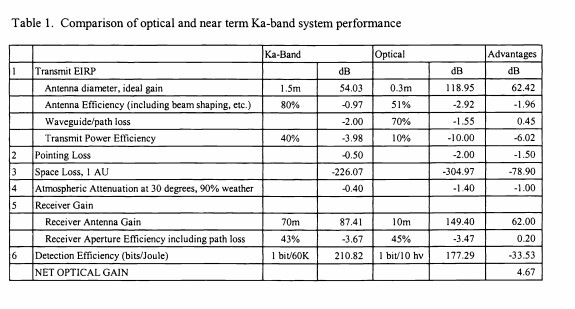
\includegraphics[width=1\columnwidth]{figures/laser-communication/bh3.jpg}
\caption{Comparison of optical and ka-band system performance}
\end{center}
\end{figure}
\noindent
Shown in Table 1 is the performance comparison between the proposed optical link and a near-term achievable RF link performance using Ka-band \cite{comparison}. Assuming equal power for the receiver and for monitor and control functions, the comparison is based on a constant DC power consumption by the transmit power amplifier. The optical link estimate is based on a 30 cm aperture diameter transmitter and a 1O m diameter receiver using 256-ary PPM and a I .06 jtm diode-pumped solid state laser. The Ka-band performance projection is based on the assumption that continuing improvements in Ka-band will lead to 
(a) implementation of Ka-band reception capability on the 70 m stations,
 (b) improved receiver aperture efficiency with either
the array feed or adjustable mirror technology, 
(c) improved spacecraft Ka-band transmitter power efficiency with high efficiency TWTAs, 
(d) Improved transmit aperture efficiency using off axis or displaced-axis antenna.

\subsubsection{Weather}

Despite of many such technological development, the major limitation of free-space laser communication (lasercom) performance is the atmosphere.  Atmospheric condition ultimately determines the laser communications systems pe for uplink-downlink , because a portion of the atmospheric path always includes turbulence and multiple scattering effects.
Heavy fog is a major weather constraint that almost completely blocks sources of light. Thus, it threatens FSO (Free-space optical communication) links by attenuating the light signal and almost breaking it.
 Light can be absorbed into the atmosphere. The phenomenon of absorption is caused mainly by the presence of water vapor and carbon dioxide in the air. These gases in addition to other types create what is called transmission windows that limit the passage of some light frequencies. The frequencies of laser sources are not in the range of absorption by these transmission windows, resulting in no effect on the communications link. laser sources are not affected by the atmospheric absorption of light during the transmission and receiving process.
Scattering is more of a concern to FSO links than absorption. This is true because scattering is a function of the light wavelength and the quantity and size of scattering elements in the atmosphere. scatter FSO light sources but the effect is considered negligible. The main weather contributor to signal attenuation is fog. Fog occurs when humidity of the air reaches a certain saturation level which condensates vapor to water droplets of microns of radius. These droplets are the major cause of scattering for infrared light. Even though fog droplets are smaller on average than cloud droplets but are huge when compared to the wavelength of the light.
The method of transmitting data from JIMO back to Earth is to use a free-space laser communications link from JIMO to an Earth-orbiting relay satellite. Using an optical receiver on an Earth-orbiting relay satellite is advantageous because it makes it possible to overcome the severe  atmospheric losses that may be experienced in direct optical transmission to a ground-based receiver.

\subsubsection{Proposed laser communication between Europa and earth}

The method of transmitting data from JIMO back to Earth is to use a free-space laser communications link from JIMO to an Earth-orbiting relay satellite. Using an optical receiver on an Earth-orbiting relay satellite is advantageous because it makes it possible to overcome the severe  atmospheric losses that may be experienced in direct optical transmission to a ground-based receiver. High data transmission rates can be achieved by using Wavelength Division Multiplexing (WDM) with multiple optical carriers each at different wavelengths. Additionally, a single transmitting telescope on JIMO can support the transmission of an optical beam that optically combines or multiplexes the data-modulated outputs from a multiple number of laser transmitters, each operating at different wavelengths.

Transmit optical aperture diameters ranging from 30 cm to 90 cm are evaluated. A single receiving telescope on the Earth-orbiting relay satellite is required with an optical aperture size that must be large enough to collect a sufficient amount of propagated light from the arriving optical light beam for carrying out reliable data demodulation and decoding. Receive optical apertures of 2.4 m and 3.6 m \cite{lasercom} .

\subsubsection{Wavelength}

Selection of wavelengths for optical communications depends on an understanding of the propagation channel, both through free space and atmosphere, and on the availability of components and subsystems including lasers, detectors, and optics. Additionally, issues pertaining to availability and reliability of components, especially lasers and detectors for user spacecraft, are critical to the selection of a viable communications wavelength. Considerations of missions and operational issues can also profoundly affect the choice of wavelength. Free space propagation loss decreases with wavelength, and provides the single most compelling reason to choose shorter wavelengths for laser communications. The angular beam diameter for a diffraction limited beam as measured by the first Airy disk of the diffraction pattern for a circular aperture is given by 2.44 $\tfrac{\lambda}{D}$, where D is the diameter of the transmitting aperture and $\lambda$ is the wavelength. Energy density at the receiver is inversely proportional to the square of the beam diameter. For a given distance z and transmitting aperture, the received energy density increases as $\lambda^{-2}$ below Fig., shows that the energy density decreased by three orders of magnitude as the wavelength increases from 0.4 to 12.5 micro m. This provides a strong argument to choose shorter wavelengths for laser communications \cite{article:wavelength}.
\begin{figure}[htb]
\begin{center}
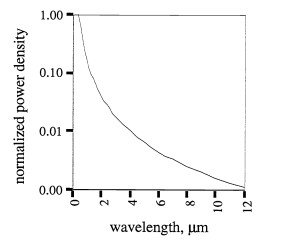
\includegraphics[width=0.7\columnwidth]{figures/laser-communication/bh4.jpg}
\caption{wavelength and power density}
\end{center}
\end{figure}
\\
We propose to use wavelengths on the ITU (International Telecommunication Union) grid specified for terrestrial fiber networks in the C band with nominal wavelengths between 1.53 and 1.57 microns (5 THz bandwidth). This choice of wavelengths takes advantage of the extensive terrestrial fiber network WDM technology currently available, including laser sources, photodiode detectors, erbium-doped fiber amplifiers (EDFA) for optical amplification, and WDM multiplexers and demultiplexers. 

\subsubsection{Modulation Type}

The large geometric space loss for communicating with deep space optical missions such as JIMO requires power efficient communication techniques.
optical detection receiver, is proposed to provide a highly power-efficient high data transmission rate system with reasonable implementation complexity. Specifically, a 256-slot PPM modulation scheme with RZ pulse shaping is considered, where each symbol carries 8 bits, requiring a 32-fold bandwidth expansion relative to the conventional binary on/off keying modulation normally employed in terrestrial fiber networks.

\subsubsection{Laser Source}

A high-power laser source at each wavelength can be implemented using a conventional laser diode followed by an EDFA power amplifier to produce 5 watts of launch power. Link closure at a 1.55-micron wavelength is then achieved for a 2.4 m receive aperture at data rates ranging from 2.5 Mbps for a 30 cm transmit aperture to 25 Mbps for a 90 cm transmit aperture. Increasing the receive aperture to 3.6 m increases the corresponding data transmission rates.

\subsubsection{Tx and Rx Aperture}

A single receiving telescope on the Earth-orbiting relay satellite is required with an optical aperture size that must be large enough to collect a sufficient amount of propagated light ,As we can see, the total telemetry data rate increased by increasing the transmitter aperture and receiver aperture, and adding more laser diode will increase the data rate. 
\begin{figure}[htb]
\begin{center}
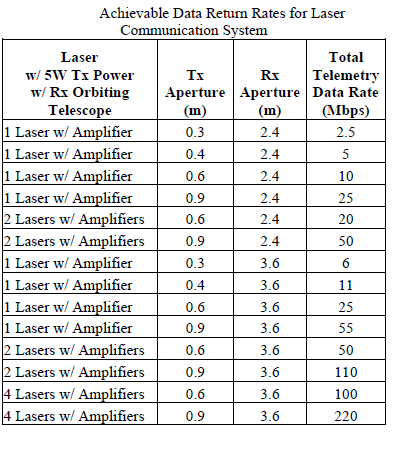
\includegraphics[width=0.7\columnwidth]{figures/laser-communication/bh5.png}
\caption{Achievable Data Return for laser Communication System}
\end{center}
\end{figure}
\\

\subsubsection{Pointing system}

Due to high data rates and reliability, the stability of the laser beam pointing is still a key technique which needs to be solved; otherwise, the beam pointing jitter noise would reduce the communication quality or, even worse, would make the inter-satellite laser communication impossible. 

\subsubsection{Weight, size, and power requirements}

The weight, size, and power requirements for a JIMO transmitter employing two wavelengths are estimated using extrapolation from previous work performed at The Aerospace Corporation.
\begin{figure}[htb]
\begin{center}
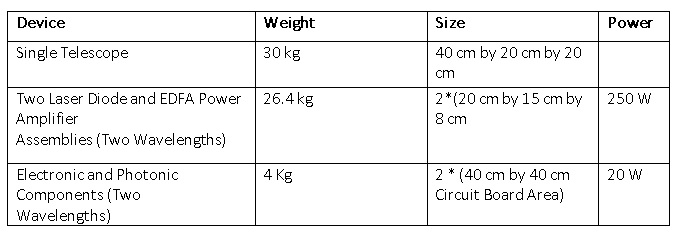
\includegraphics[width=1\columnwidth]{figures/laser-communication/bh11.jpg}
\caption{weight, size, and power requirements}
\end{center}
\end{figure}
\\

\subsubsection{Mission and Coverage limitation}

For almost all deep space missions, the mission profile will impose limits on spacecraft attitude and pointing of spacecraft during certain mission phases. Examples of such mission phases are the launch phase or inner cruise phase where spacecraft attitude is constrained by the trajectory or thermal consideration.there will be coverage holes that can potentially limit the mission planning.
-Difficulty in maintaining link with degraded spacecraft performance: This can include degraded station-keeping capability, degraded star tracker performance, or loss of time reference, will lead to unmanageable acquisition time.

The detection sensitivity is significantly worse at optical frequency, even with the use of high order PPM modulation . The optical receiver sensitivity can further degrade to 20-30 photons/bit under daytime conditions with current receiver technology.

Due to a high distance and difficulty of continuous acquisition and tracking, we can not use laser communication for this mission.


\autsection{Surface-to-Orbiter}{Rasmus Lundby Pedersen}
As it was discussed in the section covering the initial considerations associated with the full communication system, it was decided that using the orbiting satellite as a relay-station, in stead of transmitting data directly to and from earth to Europa, was a viable solution for the collective communication systems design.\\
This section will focus on the considerations concerning the design of the antenna system, the losses tied to the system and the surrounding environment, limitations, and required power for the data transfer between the surface of Europa and the orbiting satellite.

\subsection{Considerations and General Assumptions}
There are several critical considerations tied to the design of a communication link between two antennas. For space applications, these generally include, but are not necessarily limited to:

\begin{itemize}
\item \underline{Transmission distances and relative loaction.} A critical parameter of the design is the distance that the transmitted data signal must travel between a transmitter and a receiver. This aspect governs part of the required power usage (and in turn, the antennas' gains), while a target antenna moving with reference to the transmitting antenna may require tracking capabilities to be installed. Of course, the last point will depend on the available power and gain of the antennas.
\item \underline{Atmospheric Environment.} Losses in the systems varies greatly with the environment in which the transmitted signal must travel. Electromagnetic waves will always see losses when travelling in free-space, or at least near-vacuum, but will be significantly attenuated if for example they are travelling in a thick atmosphere like our Earth's.
\item \underline{Structural restrictions.} Ground-based antennas usually have very few space-restrictions, and can often thus be very large. However, when designing a system for a satellite, or an extraterrestrial exploration mission, the volume and mass of the product must be kept as an absolute low. Larger antennas are in some cases synonymous with higher gain (See parabolic antennas), so there will often be a trade-off here.
\end{itemize}

Smaller, more specific aspects should also be included in the considerations, such as the size of the transmit windows as well as the bit-rate of the transmitted data.\\
\\
We currently believe Europa has an almost negligible tenuous oxygen atmosphere, which is a major advantage in the power-calculations in the final link-budget, since we can assume that $\mu\approx\mu_0=4\pi\cdot 10^{-7}\,\mathrm{Hm^{-1}}$ and $\epsilon\approx\epsilon_0=8.854\cdot 10^{-12} \,\mathrm{Fm^{-1}}$ for the atmosphere \cite{SciStrat}. Further studies of the Jovian moon through additional missions, like the planned CLIPPER, are required to support this theory, but it means that we can assume an signal attenuation of about $\alpha_{atmos}=2\,\mathrm{dB}$ in the atmosphere.\\
\\
The moon is constantly victim to extreme amounts of radiation from Jupiter, which is estimated to be 10 times stronger than Earth's Van Allen belts. One consequence of this is, that any electronics parked in a region illuminated by this radiation would be destroyed immediately. Another, is the massive radiation noise picked up by the antennas, which would effectively render the communication link useless.\\ 
We're fairly certain Europa is tidal locked to Jupiter, which means that roughly the same side of the moon points toward the planet at all times, with a small derivation through time. This feature will likely be utilized by landing the penetrator module on the anti-Jovian side of the moon. This way, the comm-link will constantly be shielded by the moon itself, and the radiation noise from Jupiter can be neglected. An article written by 3 undergraduate students from the University of Texas state that they would expect having to transmit through a Jovian radio noise of $T_{ant}=2000\,\mathrm{K}$ \cite{DORRA}, in the S-band. However, it's unsure if they intend to operate on the anti- or pro-Jovian side of the moon, and we're not sure where they have obtained the noise temperature numbers from. Therefore, a noise temperature of $T_{ant}=200\,\mathrm{K}$ will be used, since this is often considered as the cosmic background noise-level in the S-band.\\
\\
We expect the round-trip time of the relaying satellite's orbit around Jupiter to be around 13 Earth days. During those 13 days, data from the instrument suite will be transmitted from the penetrator to the surface module and stored in a memory-block located in the part of the descent vehicle that had been submerged a few meters in the surface-ice, for radiation protection.\\
\\
It's fairly common for satellites to carry complimentary X- and S-band\footnote{The X-band ranges from 8-12 $GHz$, and the S-band ranges from }, low- and high-gain antennas for near-Earth passes and deeper space communications respectively\footnote{A S-band telemetry transmitter is used for the communication to Earth, in the CLIPPER mission.}. This is also due to their allocation for deep-space mission communication. In an effort to re-use some of the instruments on the satellite, the X-band low-gain amplifier will be utilized for the Surface-to-Orbiter link. This locks the carrier frequency to $f_c=8-12\,\mathrm{GHz}$, and thus the free-space signal wavelength to $\lambda_0=\frac{c}{f_c}=25-37mm$, where c is the speed of light, and will most likely govern the size of the antenna, depending on the design.
\subsection{Drivers}
We determined that the bottle-neck of the communication chain between the penetrator and Earth would lie in the thru-ice link, with it bit-rate limited at 10kbps. With a orbital round trip for the satellite of 13 days, this means that we need to transmit a data load of around $13\,\mathrm{days}\cdot 10\, \mathrm{\frac{kb}{s}}=11\,\mathrm{Gb}$ in 3 hours; an average bit-rate of $b=\frac{11\mathrm{Gb}}{3\mathrm{h}}=1\,\mathrm{\frac{Mb}{s}}$.\\
However, it may prove that the bottleneck is that this link, since the bit-rate of transmitted signal is directly proportional to the required transmitting power.\\
\\
A loose assumption was made, that the transmission window starts when the satellite is located $45^\circ$ above the horizon, when the distance between the surface module and the orbiter is around 6600km. This is the absolute worst-case scenario, since the actual distance will be much lower in the majority of the time in the transmission window. The link budget is calculated for this distance in order to be sure that we can guarantee a certain standard of signal quality.
\subsection{Solution Proposals}
In this part, three solution proposals are presented, and the most suitable decided. The three chosen designs are:
\begin{itemize}
\item The parabolic antenna.
\item Phased array patch antenna.
\item Crossed dipole antenna. 
\end{itemize}
Design and production costs are not considered for the three solutions. 
\subsubsection{Parabolic Antenna}
The parabolic antennas are typically used for ground station antennas and on satellites with well-known and reliable attitude orientation, with respect to its target.\\
A main advantage is it's considerable antenna gain, which is given by:
\begin{equation}
G = \eta_a\left(\frac{\pi D}{\lambda}\right)^2
\end{equation}  
Where $\eta_a$ is the aperture efficiency, typically ranging between $0.55<\eta_a<0.7$, D is the circular diameter of the parabolic dish and $\lambda$ is the signal wavelength.\\
It can be seen that the gain of the antenna is directly proportional to its size, which itself is independent of the signal's wavelength. This means that the antenna can be scaled for the desired gain, within structural limitations. 
\iffalse
An example could be a small antenna with a dish diameter of $D=1\,\mathrm{cm}$, used in the X-band ($\lambda_0=30\,\mathrm{cm}$ with an efficienty of $\eta_a=0.6$:
\begin{equation}
G=0.6\cdot\left(\frac{\pi\cdot 1\cdot 10^{-2}}{30\cdot 10^{-3}}\right)^2=	
\end{equation}
\fi
\\
A disadvantage of a high-gain antenna is, that must be oriented towards its target with fairly high accuracy. This can be achieved by mechanically tracking the target on the sky with motors, which in itself is un-desired for any space-related mission. Pin-pointing the target also proves difficult for a surface based station on Europa, where we are without a network of GPS satellites to track the position of the surface antenna with respect to the orbiting satellite. We have practically no way of knowing where to point the antenna, and the benefits of its large gain will be lost.\\
Of course, scaling the size of the antenna down to a lower gain is also possible, but this defeats the purpose of using the parabolic type, being it's potential high gain, and since it typically comes with a large number of undesired side-lobes in its radiation pattern. 
\subsubsection{Phased-Array patch Antenna}
The problem of using mechanical tracing for the parabolic antenna can be solved by using phased-array patch-antennas in stead. A single flat patch antenna doesn't necessarily come with a particularly impressive antenna gain, but an array of the has shown to enable us to modify its radiation pattern. Differentiating the phases between the patches will in turn make it possible to direct the radiation pattern dynamically, and the high carrier frequency allows us to reduce the size of the patch antenna significantly compared to the parabolic antenna. The principle of a phased-array antenna is shown on figure \ref{fig:phased}\footnote{\url{http://tempest.das.ucdavis.edu/mmwave/paa_files/image005.png}}.\\
\begin{figure}[!htb]
	\centering
	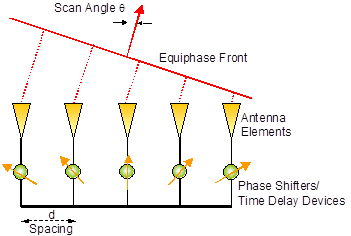
\includegraphics[width=0.5\textwidth]{figures/Rasmus/phased}
	\caption{A simplified concept illustration of the Phased array antenna .
	\label{fig:phased}}
\end{figure}
However, the issue of tracking the target on the sky still persists and remains un-solved. Therefore, it seems that the parabolic antenna and the phased-array patch antennas share the same mission-critical disadvantages.

\subsubsection{Crossed Dipole Antenna}
The third solution is using a half-wave dipole antenna for the communication link. The half-wave dipole is possibly one of the most simple antennas, often associated with a low gain of $G_{dipole}=2.15\,\mathrm{dBi}$. The design is basically a straight conducting wire with a length of $l=\frac{\lambda}{2}$, which can either be center-fed or fed in one of the ends.\footnote{In practice, the length is actually closer 0.47$\lambda$ since the resonant length depends on the thickness of the wire.}\\
\\
The radiation pattern of a half-wave dipole antenna can be seen on figure \ref{fig:singeldip}, which is only dependent on the polar angle, with respect to the horizon having the antenna parallel to the surface plane.
\begin{figure}[!htb]
	\centering
	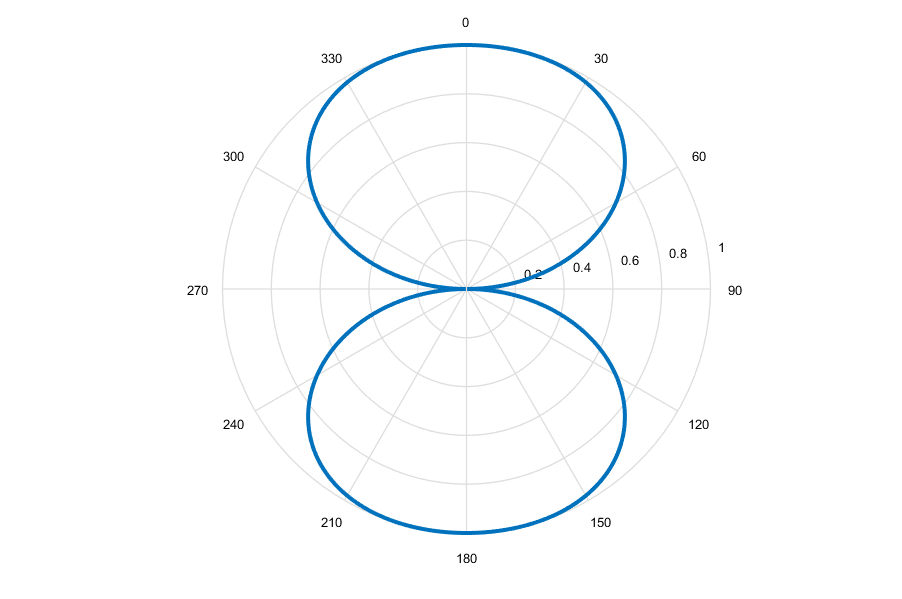
\includegraphics[width=0.80\textwidth]{figures/Rasmus/dipalone1}
	\caption{The horizontal normalized (E field) radiation pattern of a half-wave dipole antenna. The antenna elements are located along the 270° to 90° line.
	\label{fig:singeldip}}
\end{figure}
The plot clearly shows that the power is split in two directions, on either side of the horizontally oriented dipole antenna. If we consider the surface-antenna being parallel to the surface, the orbiter will be located in the upper half of the polar plot during the transmission window. Therefore, we want to reflect all of the power in its direction by placing a large conducting plate underneath the antenna. Simple electromagnetic reflection and image theory can be applied if the conducting plate's geometry is significantly larger than the electrical length of the antenna. This way, the plane can be assumed infinitely large and we will avoid wave scatterings.\\
The radiation pattern of the modified half-wave dipole will vary with the distance between it and the ground plane, due to the phase differences between the incident field and its reflection from the conducting plane. Electromagnetic theory can be applied to show that placing it $\frac{\lambda}{4}$ above the plane will result in a simple single-lobe pattern (no side-lobes) with double the amplitude of an ordinary half-wave dipole antenna. The total far-field E-field expression of the horizontal antenna is given by:
\begin{equation}
E=E^i+E^r=j\eta_0 \frac{\beta_0 I_0 l e^{-j\beta r}}{4\pi r}\sqrt{1-sin^2(\theta)sin^2(\phi)}[2jsin(\beta_0 h cos(\theta)]
\end{equation}
Where $\eta_0$ in the intrinsic wave-impedance given by $\eta_0=\frac{\mu_0}{\epsilon_0}$, $\beta_0=\frac{2\pi}{\lambda_0}$, $I_0$ is the current in the antenna, $l$ is the dipole's length, $r$ is the distance between a reference point on the conducting plane underneath the antenna and the observation point ($\lambda_0<<r$), and $h$ is the distance between the antenna and the conductive plane. $\theta$ Is in this case the polar angle from zenit to the horizon ($0-\pi\,\mathrm{rad}$) and $\phi$ is the azimuthal angle - the coordinate system can be seen on figure \ref{fig:reflect}. 
\begin{figure}[!htb]
	\centering
	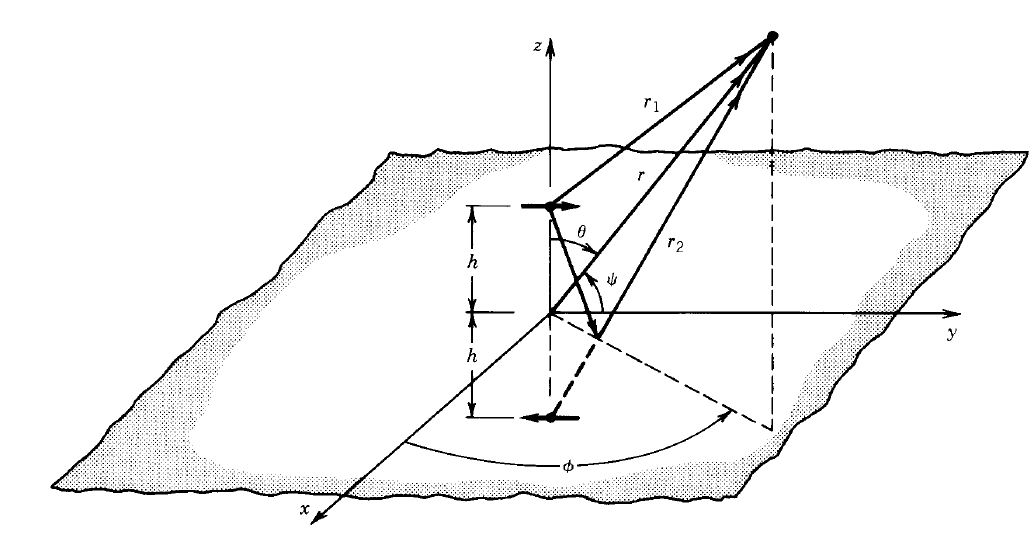
\includegraphics[width=0.75\textwidth]{figures/Rasmus/reflectCoord}
	\caption{Horizontal electric dipole above an infinite electric conductor (Source: C. A. Balanis, Antenna Theory: Analysis and Design. Copyright \textcopyright 1982, John Wiley \& Sons, Inc.)
	\label{fig:reflect}}
\end{figure}
The normalized radiation pattern, $E_{norm}=E\cdot \frac{4\pi r}{\beta_0 I_0 l}$ was calculated in matlab for $h=0$, $\frac{1}{4}\lambda$, $\frac{1}{2}\lambda$, $\frac{3}{4}\lambda$ and $\lambda$ (The script can be seen in appendix \ref{app:rasmusmatlab}) and plotted as seen on figure \ref{fig:Lobes}. The field intensity will vary with $\phi$, but the influence is practically so small for the purpose that it's set to 0.  
\begin{figure}[!htb]
	\centering
	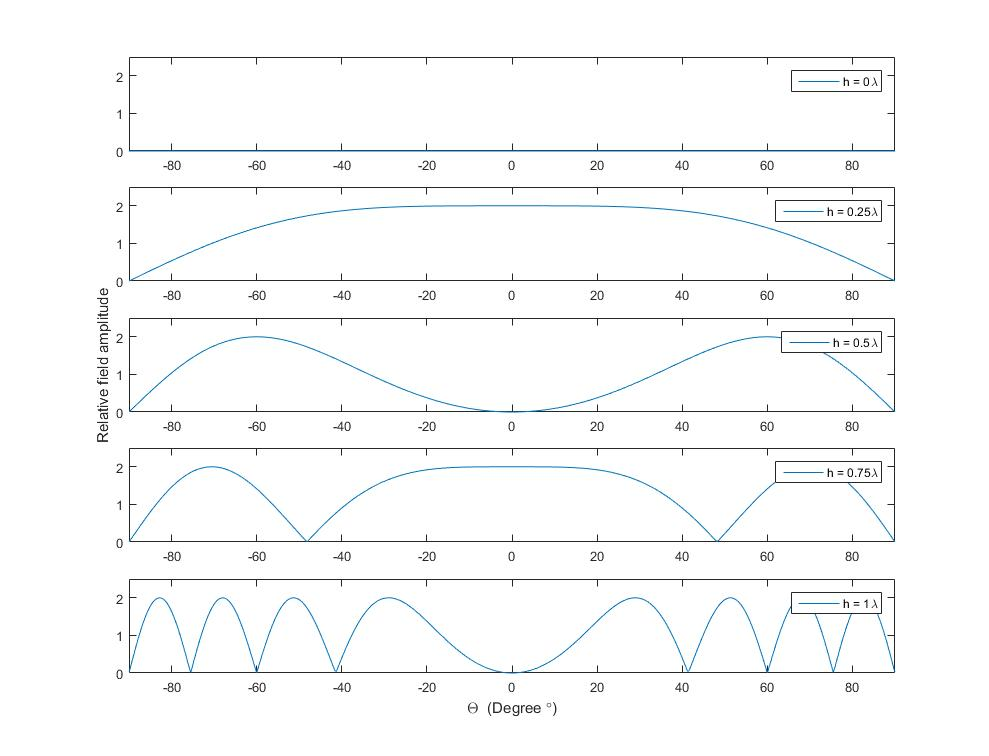
\includegraphics[width=0.75\textwidth]{figures/Rasmus/Lopes}
	\caption{Theta-variant of the radiation pattern for the crossed half-wave dipole antenna.
	\label{fig:Lobes}}
\end{figure}
It can be seen that the antenna gain retains the same radiation pattern in the upper half of the field but with twice the gain, $G_{plane}=4.15dBi$, when $h=\frac{\lambda}{4}$.\\
The same principle is applied to the antenna on the orbiter.\\
\\
Being linearly polarized, we risk to loose the signal link if the orbiter is not positioned for a maximum polarization efficiency. This can be solved by crossing the dipole antenna with another identical antenna, creating a circularly polarized antenna and thus making it omnidirectional. However, this will also cut the antenna gain in half, effectively making it $G_{crossed}=2.15\,\mathrm{dBi}$. 

\iffalse
\begin{figure}[htb]
	\centering
	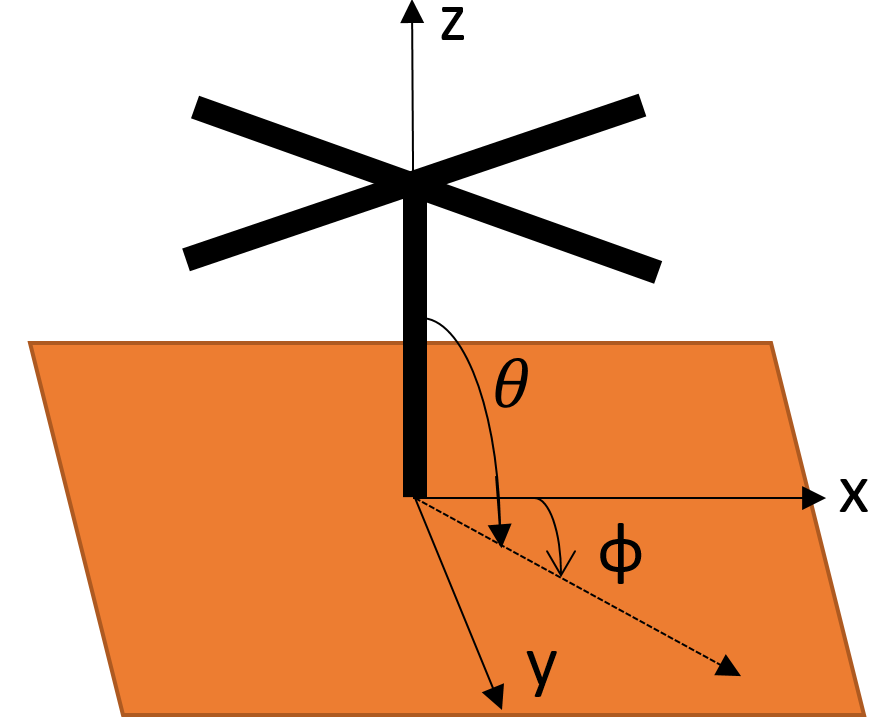
\includegraphics[width=0.6\textwidth]{figures/Rasmus/CrossDip}
	\caption{Crossed half-wave dipole antenna drawing.
	\label{fig:DrossDip}}
\end{figure}
\fi

\subsection{Implementation and Link budget}
There has been talk about mounting patch antennas on the extruding stabilizer feet on the landing module that remains on the surface, for communication through the ice to the penetrator vessel. Therefore, it may also be possible to mount crossed dipole antennas for the communication with the orbiter on each of the feet, to create a more omni-directional antenna system in case the lander doesn't rest flat on the surface. This could obstruct the line-of-sight to the passing orbiter, and having four seperate antennas to choose between would help solve this potential problem. Each dipole will have a length of $l=15\,\mathrm{mm}$, and the total communication electronics-system, including amplifiers and additional circuitry, will weigh around $m_{comm,surface}=20\,\mathrm{kg}$. The transceiver systems will be located in a radiation-protected module located a few meters in the ice, so only some wires and the antennas themselves will be subject to possible radiation on the surface.\\
Two crossed antennas will be placed on the orbiter for redundancy purposes. The exact location of the antennas should be determined in cooperation with the people designing the remote-sensing instruments, so that we're sure they're visible from the surface at all times during the communication window.\\
\\
It's typical to create a link-budget to determine the required power of transmission in the communication system, which can be seen on figure \ref{fig:surfLink}.
\begin{figure}[!htb]
	\centering
	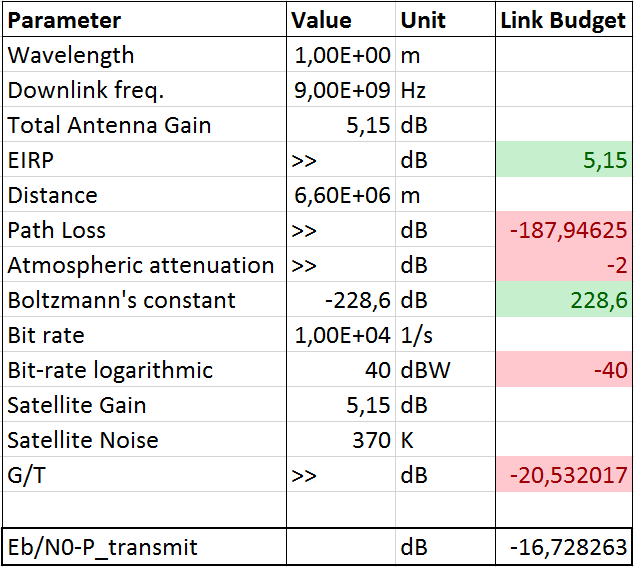
\includegraphics[width=0.6\textwidth]{figures/Rasmus/Link}
	\caption{Link-budget for the surface-to-orbiter communication link.
	\label{fig:surfLink}}
\end{figure}
The required power will depend on the encoding scheme, but we can see that we'll need $16\,\mathrm{dBm}=47\,\mathrm{W}$ of power to get a signal-to-noise-ratio of $0\,\mathrm{dB}$.\\
\\
Total mass, volume and power costs of the surface-to-orbiter communication link are given in table \ref{tab:commsurf}. Weight and mass of the antennas are omitted to their small sizes.
\begin{table}[htb]
\centering

\label{my-label}
\begin{tabular}{|l|l|l|l|}
\hline
\textbf{Unit}        & \textbf{Weight (kg)} & \textbf{Volume ($m^{3}$)} & \textbf{Power (W)} \\ \hline
Amplifier on Surface & 2                    & $0.1\cdot 10^{-3}$        & 20                 \\ \hline
Amplifier in Orbiter & 2                    & $0.1\cdot 10^{-3}$        & 20                 \\ \hline
\hline
Total                & 4                    & $0.2\cdot 10^{-3}$        & 40                 \\ \hline
\end{tabular}
\caption{Total mass, volume and power costs of the surface-to-orbiter communication link}
\label{tab:commsurf}
\end{table}
The power and weight costs seem to be within reasonable ranges. 
\subsubsection{Future Work}
\iffalse
There are two major subjects that could be investigated in the future for preparation of the mission.\\
\\
\fi
A more detailed link-budget could be achieved if we assumed that the transmission power could be varied with distance between the surface-module and the orbiter during the transmission window. As of now, we assume a worst case scenario with a distance of $6600\,\mathrm{km}$, but this is not a realistic value. The actual required power tied to this distance will be significantly lower.\\

\iffalse
1. Introduction and considerations for the link
      * (Orbit characteristics and Europa Environment)
1. Link Drivers
   1. Radiation (Europa surf dead zone)
   2. Low Power
   3. Transmission Relay Window
      * Dataload
      * Bitrate
   1. Low Temperature Operation
   2. Line of Sight (viewing angles)
      * Communication while descent maneuver
      * Antenna choice
      * Mechanical stabilizers
1. Link Budget
2. Solution Proposal
3. Drivers to other systems
\fi



%   Include in Comm Systems
%   target 8-10 pages
\autsection{Penetrator-Lander Link}{Gustavo Feijóo Carrillo}
%   Through Ice Communications
%       -Scenario and description of operations
%       -Communications during descent
%       -Propagation through ice, ice losses
%       -Link necessary capabilities
%       -Possible hurdles

\paragraph{Link scenario and description of operations}
Three stages in the process of the penetrator descending through the ice crust can be defined to better design the communication system. First, the deployment of the vehicle by lowering it by means of a controlled crane system. In this phase a critical mission operation must be carried out, this is the burial of the lander computer and electronics subsystem to protect it from the surface heavy radiation doses which would shrink the mission life to about a month making it impossible to reach the ocean and carry out the mission goals.

The second phase, would be the penetrator complete buried within the crust and on the melting process to reach the ocean, this might be the longest duration stage depending on the thickness of the crust at the landing site. In this phase, a big risk is the effect of the "slushy" ice trail behind the penetrator. This watery ice would have an increased conductivity and it poses as an obstacle in the path of communication from the penetrator vehicle to the lander. This obstacle mainly affects the antenna pattern characteristics but its effect is greatly dependant on the dimensions of the "slushy" ice trail. On the other hand, a tethered solution would be driven by cable mass necessary for depth goals and to withstand the mechanical forces from being frozen in the ice crust, specially the shear stresses (from sideways motion of ice sheets).

Third, reaching the ocean interface where the main transceiver in the penetrator is left embedded at a safe distance from the interface with the anchoring mechanism for the penetrator and instruments suite. A tether enabled for communications will serve as link from the instruments to the main transceiver and relay the science data and telemetry to surface.

\begin{figure}[htb]
	\centering
	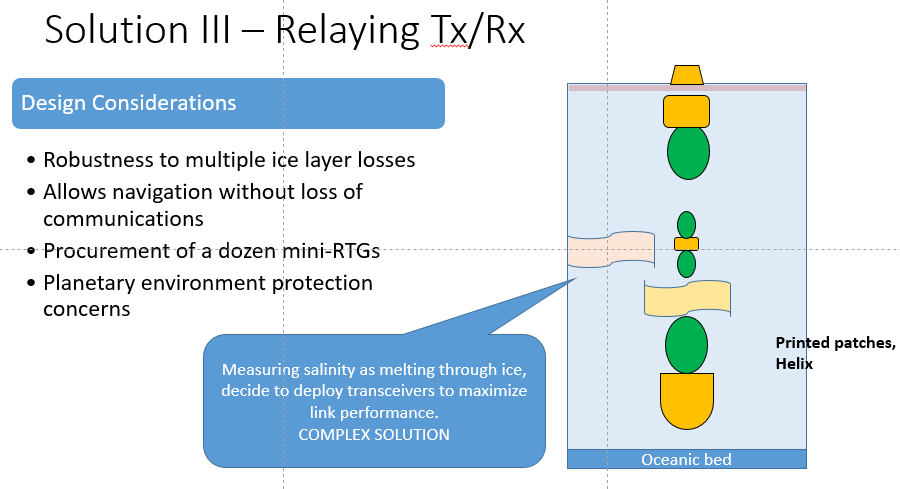
\includegraphics[width=\textwidth]{figures/comms/iceLink-relay}
	\caption{\textit{DRAFT} Through-ice communications.}
	\label{fig:through-ice_comms}
\end{figure}

\subsection{Link Drivers}

\autsubsection{Tethered Link}{Kristian Sloth Lauszus}
One option for the penetrator to surface communication would be to use a tethered link connected from the end of the penetrator to the surface station. For instance a optical fiber could be used. The main benefit when using optical fiber for communication is the huge data rate of 10 Gb/s and beyond, which will allow the penetrator to broadcast scientific data, images and even video to the lander. Another advantage is that it is not unusual for optical fiber communication to work at up to 100 km without the need of any amplification\cite{website:optical_fiber_info}, which is way more than the worst case scenario of 36 km, as described in chapter \ref{sec:structural_profile}. Thus the optical fiber is very interesting, as it will basically allow one to send all the scientific data to the lander with little to any concerns about the data rate.

\subsubsection{Optical fiber strain}

However one major concern is whenever the strain from the ice caused by the tidal waves will exceed the capabilities of the fiber and eventually break it. This will be discussed in detail in the following section.\\

\noindent
According to Hook's law the force along the longitudinal axis of the optical fiber is given by:
\begin{equation}
	 F = k \, \Delta l
\end{equation}
Where $k$ is the elastic constant of the optical fiber and $\Delta l$ is the relative deformation caused by the perturbation force $F$. This law is fulfilled as long as the deformation does not exceed the elastic limit of the optical fiber which will prevent the fiber from retracting back to its original shape.

By knowing the Young's modulus of the optical fiber once can calculate the force of the perturbation using the following formula:
\begin{equation}
	F = E_G \, A \frac{\Delta l}{l}
\end{equation}
Where $E_G$ is the Young's modules, $A$ is the area of the optical fiber and $l$ is the length of the optical fiber.

By measuring the force applied to an optical fiber and plotting it versus the strain one can estimate the Young's modulus at the point where the slope of plot is no longer linear. Furthermore this point will also indicate the maximum strain of a given optical fiber. This strain number is very useful in our case, as this tell us how much the fiber can stretch before it is degraded. A typical number for protected optical fiber is about 3-5 percent\cite{article:optical_fiber_properties,article:optical_fiber_mechanical}. Since the column above the penetrator will start to freeze up again it is very important that the vertical strain of the ice does not exceed this critical value, as this will cause the optical fiber to break.

\subsubsection{Discussion}

Fortunately the vertical strain of the ice sheet on Europa is only estimated to be 0.3 \%, however this does not take into effect any potential cracks that occurs at the ice surface, as described in chapter \ref{sec:surface_studies}. This might cause the ice to shift horizontally, thus risking to break the cable. Thus the tethered link is very risky and should properly not be used as the only form of communication\cite{book:communication}.

The optical fiber could be wound up on a spool with a total weight of only a few kilograms\cite{book:communication}. However the wheel will also add up in complexity of the system and increase the volume. There will also be a risk of the wheel getting stuck while unwinding the optical fiber. Another option would be to use even more rigid cable, but this will increase volume and mass significantly\citet{iceLink-scott}.


\autsubsection{Ice embedded Repeaters link}{Kristian Sloth Lauszus}

Another option for communicating between the penetrator and the lander would be to use multiple transceivers that would get deployed at certain intervals by the penetrator, as it is described by \citet{iceLink-scott}. Thus a series of repeaters was proposed, designed into 10 cm diameter cylinders with a height of 2-3 cm. Each repeater would have a 1 GHz patch antenna in the top and bottom of the cylinder and contain all the needed hardware for transmitting and receiving the data including a RTG for power and heat. Each repeater could also have temperature, pH, salinity, hydrophones and various other sensors embedded.

In the study the goal was to have a data rate of 10 kHz at 400 mW through a 10 km ice crust. In the paper the number of repeaters was found to be heavily influenced by salinity of the ice and temperature profile used. Thus the number of repeaters would increase in salty ice and if a layered ice temperature profile is used compared to a linear ice temperature model (see chapter \ref{sec:IceTemperatureProfile} and \ref{sec:IceTemperatureProfile2}). In the paper the salty ice is assumed to contain 13 PPM (Parts Per Million) salt impurities. For the linear ice temperature model the minimum amount of repeater was found to be 4 for a ice thickness of 3.5 pure ice, while 14 transceivers would be needed for 10 km salty ice. While the number of repeaters needed for the layered ice temperature profile would be vary from 8 for 5 km and 34 for 20 km pure and salty ice respectively.

However as \citet{iceLink-scott} also points out the distance between the receivers could be increased at the cost of a lower data rate, thus if the ice ends up being thicker or more salty than first expected, this could be compensated for by the on-board computer in the penetrator. On the other hand if the ice is more pure the distance could be increased or the data rate increased.

One way for the penetrator to deploy the repeaters would be to make the repeaters buoyant in such a way that they would float upward and align themselves in such a way that the antennas point up and down. A new repeater could then be deployed when the signal strength drops below a certain threshold. One problem with using the repeaters is that the complex dielectric permittivity increase in the order of 1000 times in water compared to ice, thus the penetrator might have to sit and wait for the repeater to freeze if a minimum data rate is needed.

Another option would be to use the repeaters at the outer ice crust where the ice is colder and the risk of fractures in the ice is higher, then once the penetrator gets below a certain depth a tether could be used to connect to the last repeater deployed at the warmer inner ice, where the risk of a tether breaking is less. This is especially useful if the layered ice temperature profile ends up being close to reality, as the temperature of the ice increases significantly in the beginning of the ice sheet, as discussed in chapter \ref{sec:IceTemperatureProfile2}. However then further studies would be needed in order to get more certainty regarding the ice temperature profile of Europa. Also further studies are needed regarding the salinity, as it is critical in order to estimate the number of repeaters needed.


% Wireless links
\autsubsection{Ice embedded wireless communications}{Gustavo Feijóo Carrillo}

From a previous study for JPL's Cryobot regarding ice communications \cite{iceLink-scott}, we find the assumption of the communication transceiver being allowed to refreeze in the ice but there is no deeper details on this matter. The main subject here is the behaviour of the "slushy" or water and ice mixture above the descending penetrator, since this trail has a meaningful effect on the antenna performance of the penetrator communication subsystem as we show in Figures \ref{fig:unaffected}, \ref{fig:smallSlush} \& \ref{fig:bigSlush}.

\begin{figure}[htb]
	\centering
	\subfloat[]{
		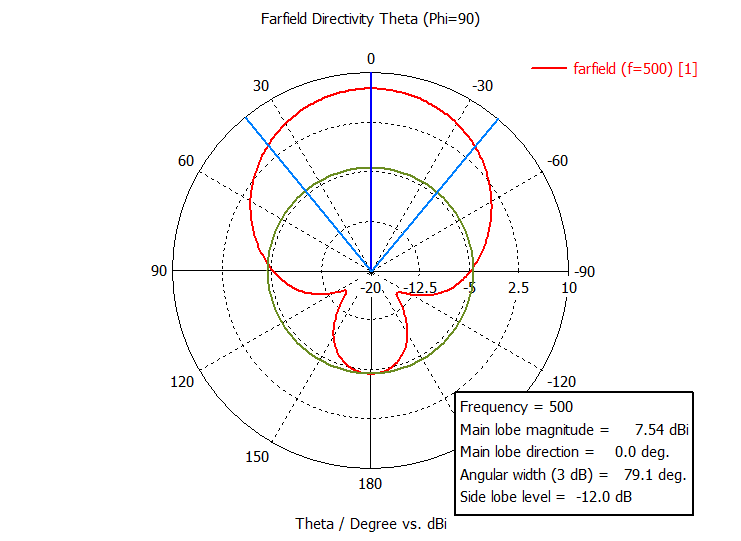
\includegraphics[width=.48\textwidth]{figures/comms/antPattern-cPatchRadome}
		\label{fig:antPatt-patchRadome}
	}
	\subfloat[]{
		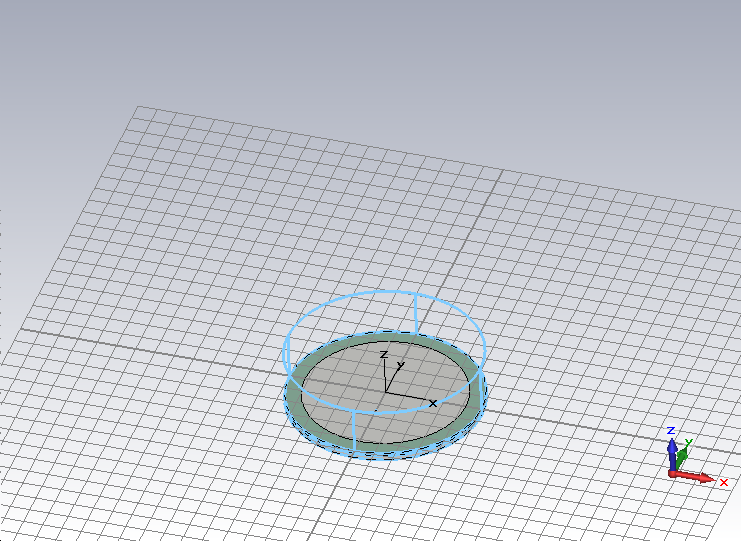
\includegraphics[width=.48\textwidth]{figures/comms/component-cPatchRadome}
		\label{fig:comp-patchRadome}
	}
	\caption{Unaffected antenna pattern.}
	\label{fig:unaffected}
\end{figure}

\begin{figure}[htb]
	\centering
	\subfloat[]{
	    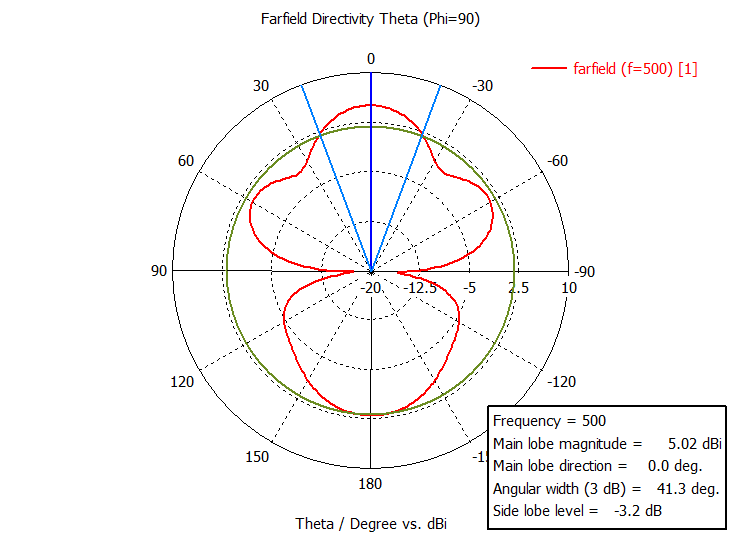
\includegraphics[width=0.48\textwidth]{figures/comms/antPattern-slushEffect-a}
	    \label{fig:slushEffect_a}
	}
	\subfloat[]{
		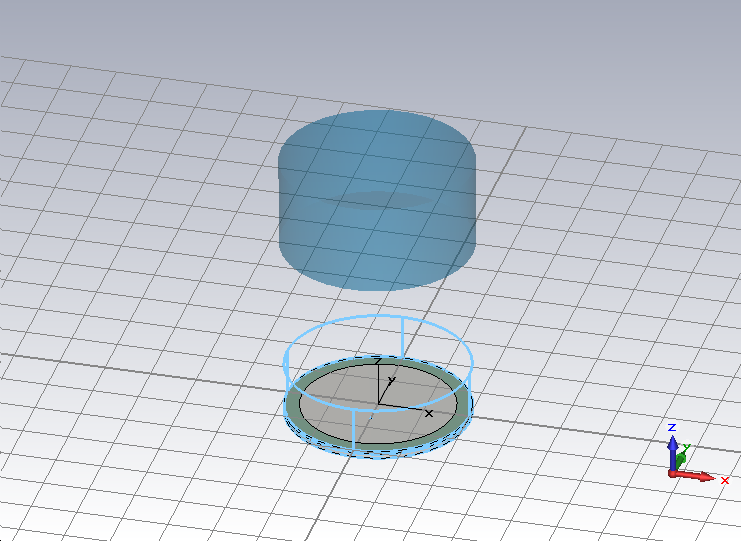
\includegraphics[width=.48\textwidth]{figures/comms/component-slushEffect-a}
		\label{fig:comp-smallSlush}
	}
	\caption{Effect of small watery ice obstacle in antenna path.}
	\label{fig:smallSlush}
\end{figure}

\begin{figure}[htb]
	\centering
	\subfloat[]{
	    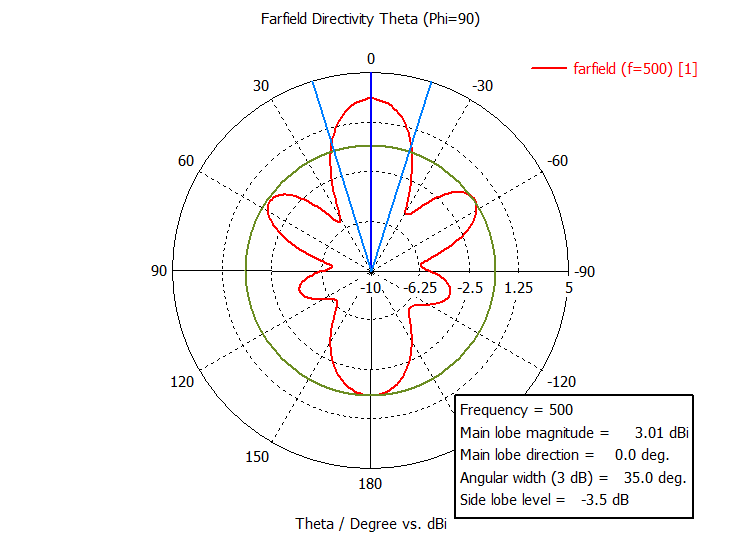
\includegraphics[width=0.48\textwidth]{figures/comms/antPattern-slushEffect-b}
	    \label{fig:slushEffect_b}
	}
	\subfloat[]{
		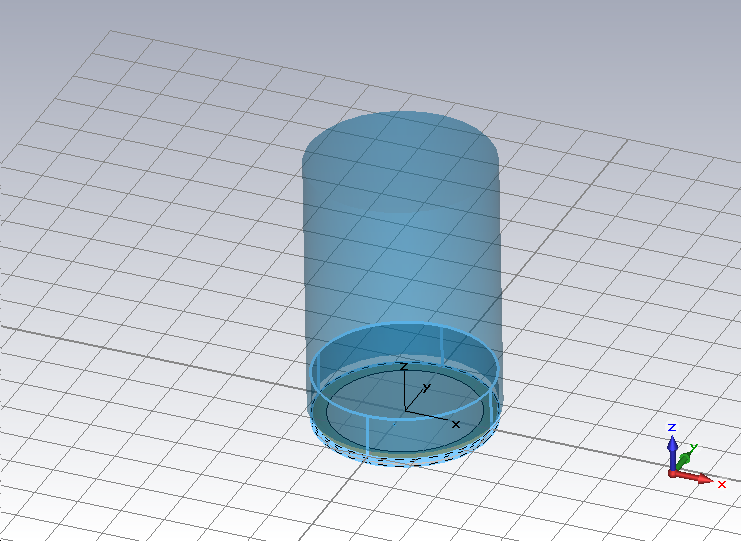
\includegraphics[width=.48\textwidth]{figures/comms/component-slushEffect-b}
		\label{fig:comp-bigSlush}
	}
	\caption{Effect of longer watery ice trail.}
	\label{fig:bigSlush}
\end{figure}


% HD link
\autsubsection{High Directivity Link}{Ioannis Nisopoulus}

\begin{figure}[htb]
	\centering
	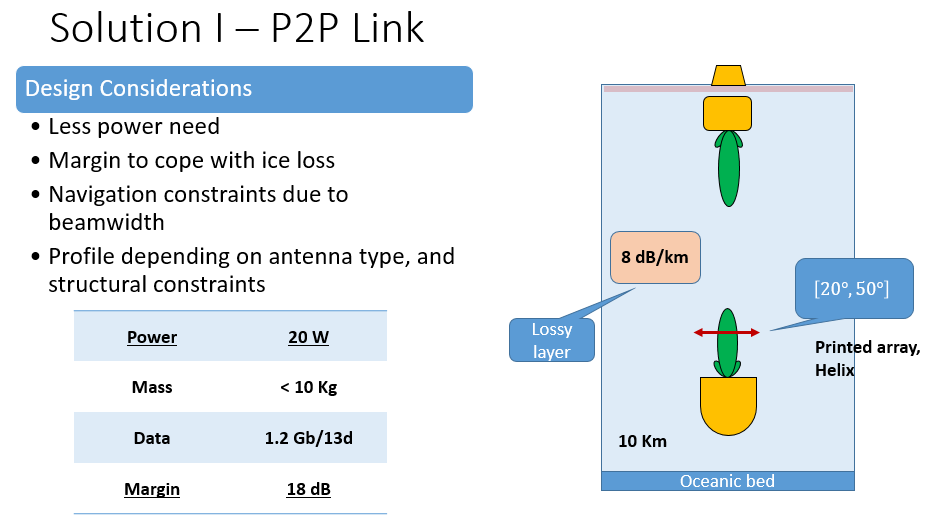
\includegraphics[width=\textwidth]{figures/comms/iceLink-p2p-HighD}
	\caption{ \textit{DRAFT} Sol I.}
	\label{fig:iceLink-p2p-HighD}
\end{figure}

%\autsection{Highly Directional Link}{Nissopoulos Ioannis}

\subsection{Link Description}

\paragraph{Directional antennas}
Directivity is a fundamental antenna parameter, which measures how much power radiated or received in a specific direction from the antenna. A directional antenna is the exact opposite of an omni-directional antenna, which transmits or receives equally from all directions. Directional antennas provide increased performance and reduced interference from unwanted sources, because of their construction and their basic principles. Well known applications for high directional antennas are among others NASA's Deep Space Network (DSN), terrestrial communication links, such as satellite television and cellular repeaters, where high position accuracy and propagation in long distances are needed. In general, high directional antennas are used in every application where high data rates, high gain and reduced interference is mandatory.

The main principle of directional antennas is their ability to concentrate almost all the transmitted power to small beamwidths, instead of illuminating wider solid angles. Saying that, they do not sacrifice any power to unwanted directions, but achieve high gain (more than 10 dBi) for specific solid angles. On the other hand, high directional antennas can reach their targets only through very narrow beamwidths, which can be a significant bottle neck in many applications and especially when tracking in long distances is required. 

Typical types of directional antennas are parabolic antennas, helical antennas, yagi antennas, horn antennas, phased arrays, etc. Directivity and gain of such types of antennas can be affected from many different parameters, regarding their type and application. The number of elements and their spacing, their physical or synthetic aperture, their surrounding environment and the manufacturing material are some of the major criterion that can change the performance of a highly directive antenna considerably. 

\paragraph{Solution description}
In this subsection we will examine if it is possible to use a high directional link for the communication segment between the lander vehicle and the penetrator of our mission. The advantages and disadvantages will be analyzed thoroughly and finally an assessment of this possibility will take place. 

The aforementioned idea is based on a pair of highly directive antennas, which can be used to achieve high rates of data streams and a stable communication channel. One antenna will be installed on lander vehicle's bottom surface looking downwards, while the other one will be placed on the top surface of the penetrator facing upwards, towards the first antenna. The line of sight between these two antennas must always be free of obstacles and we must assure that the beamwidths of the antennas are aligned and cross each other all the time. \textbf{pic} Different types of antennas will be examined in order to find out which one them is the most efficient for the requirements of our mission.

\paragraph{Drivers of Comm Link}
The design of a communication link in an inhospitable environment as Europa's subsurface can be proved especial demanding and difficult, but definitely will not be our only limitation. Space and power consumption is most of the times the number one drivers in all remotely controlled missions. The first priority when an engineer designs a communication link is the selection of the frequency range for the specific mission. In order to do so, engineers have to take into account a lot of factors such as the host environment and the attenuation that implies, the desired bandwidth, the amount of data with the corresponding data rates, etc. 

As we expect, Europa's subsurface consists of several kilometers of ice, which is a factor that limits our choice of frequency range. As described in subsection \ref{sec:ice_losses}, the longer the wavelength we use the better penetration through the ice crust we can achieve. In other words, as we go down in frequency our losses due to ice layers are diminished. Longer wavelengths are also more effective against attenuation due to impurities, because the dimensions of these impurities particles (sulfates, debris rocks, etc.) expected to be in order of millimeters. Nonetheless, the frequency of an antenna is always bonded to its size, by means that lower frequencies correspond to bigger size of antennas. Having in mind our requirements for high directivity, gain and satisfying bandwidth we must keep the size of our antenna reasonable. Other parameters that affect this size can be the type of the antenna. Moreover, due to the limited available space we will provide ways to fold and deploy the antennas wherever it is necessary.  

% \textbf{Obstacles in the near field}

\subsection{Implementation}
In this paragraph, we will examine different type of antennas for the lander vehicle, but also for the penetrating vessel. The main criteria for choosing an antenna type are the size and the ease of folding and deployment, the providing gain and the beamwidth or directivity of the antenna. Other characteristics under examination will be the capability of steering, mechanically or electronically, and the achievable data rates. After the determination of the above, we will perform the link budget analysis for the specified link. 

At first, we will concentrate only on the lander vehicle's antenna and in the next part on penetrator's. In figure \ref{fig:J_spec} can be seen the highest frequency, which is free of Jupiter's radio emissions and it is around 50 MHz, thus this is the lowest frequency choice we can make. The wavelength of this frequency is approximately 6 meters, which is way bigger than 1 meter which is the estimated available space we have under the "belly" of our land vehicle. In order to overcome this problem, we will investigate the case of a slightly higher frequencies, above 150 MHz. 

Firstly, we will present the candidate types of antennas, which will be mounted beneath our lander vehicle. It is difficult to analyze all the different types of directional antennas in the context of this report, thus we will examine three major antenna's "families", which fulfill the requirements discussed above. The first antenna type is Yagi-Uda (or Yagi) antennas together with the log periodic dipole array (LPDA). The former are used mainly from radio amateurs and they are inexpensive but quite efficient antennas for lower frequencies. A distinctive characteristic of Yagi antennas is that their design and construction based most of the times in experimental measurements hands-on experience, rather than well documented formulas and heavy mathematics. Many radio amateurs share their experience and design characteristics in order to improve the basic design as Shintaro Uda and Hidetsugu Yagi had designed in 1962. The later are a special type of antennas, which are quite similar in design with Yagis, although their distinctive characteristic is the very broad bandwidth. Because of this LPDAs are used in UHF terrestrial TV, HF communications, EMC measurements etc.

\paragraph{Yagi-Uda Design}
Yagi-Uda antennas consist of a single driven element connected to the transmitter or receiver and additional parasitic elements. The parasitic elements operate by re-radiating their signals in a slightly different phase in relation to the driven element. In this way the signal is reinforced in some directions and cancelled out in others, so a high directivity is achieved. The length and the spacing of each parasitic element determined by the operational frequency, as well as the total length of the antenna. As it can be seen in figure \ref{Yagi}, a Yagi antenna is linear polarized, parallel to its elements dimension. This is a significant drawback of this design in case the user needs to exploit different polarizations. The solution to this can be the "crossed" Yagi-Uda antenna, which practically is two antennas with two orthogonal polarizations on the same boom. Crossed Yagis provide the capability to receive or transmit in circular polarization with a -3 dB trade off of your signal. If we finally will choose this antenna type for sure we need to consider the crossed version, because the received polarization will have been rotated randomly from the ice crust. LPDAs may look similar to Yagis, although their main principle is quite different. They consist of a number of dipole elements as well, but not all antenna elements are active at any given frequency. In other words, we can imagine a LPDA as an array of dipoles tuned in different frequencies and this is the reason why these antennas hold bandwidth more than few GHz. Another difference is that the main beam of this antenna comes from the "shorter" front. LPDAs used because of their wide bandwidth and not so much because of their gain or their bandwidth. For our purposes, this antenna type will not present so many attractive points, so we will not cover them thoroughly. 

\begin{figure}[htb]
    \centering
    \captionsetup[subfigure]{width=0.45\textwidth}
    \subfloat[A typical Yagi-Uda antenna with 3 directors, 1 driven element and 1 reflectors]{
        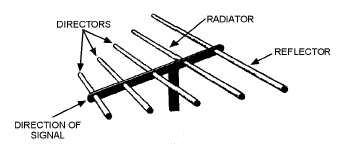
\includegraphics[width=.48\textwidth]{figures/Yannis/yagi.jpg}
        \label{Yagi}
    }
    \subfloat[The basic components of a log periodic dipole array. The forward direction is to the left in this sketch]{
        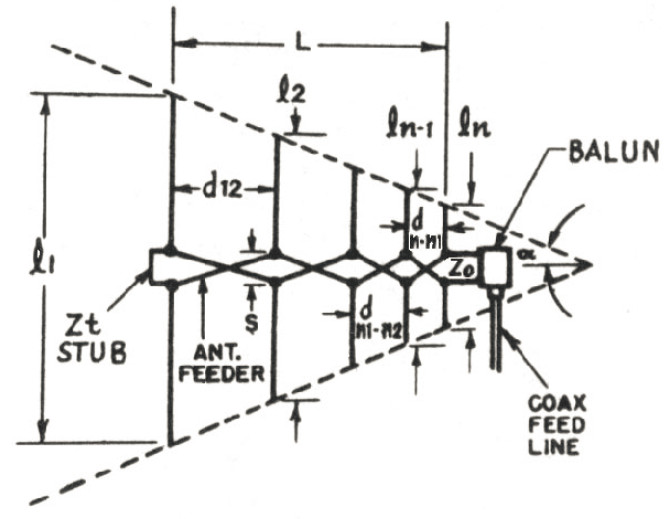
\includegraphics[width=.48\textwidth]{figures/Yannis/log2.jpg}
        \label{log}
    }
    \caption{}
\end{figure}

As it is mentioned above, the design of a Yagi-Uda antenna is usually approached with an optimization algorithm based on already existed designs. Mentioning that, the free software "Yagi Calculator" (from VK5DJ radio amateur, \url{http://www.vk5dj.com/yagi.html}) was used, which simulates the antenna and has as an output its gain, beamwidth, antenna length, etc. Our major bottleneck using Yagis will be first of all their boom length. According to many designs, the boom length should be at least 2.2 $\lambda$ in order to achieve the best performance out of the antenna. Our available space is approximately 1 meter, thus our antenna boom should be less than one meter, which corresponds practically to frequencies higher than 600 MHz. As it is clear, frequencies higher than 400 MHz present excessive losses and is impossible to be used for our application. Although, we can decrease boom length according to our desires with a trade off in gain and beamwidth. Another issue that we must take into account is the really close distant of ice from the tip of our antenna. This mean that the ice will be inside the near field of our antenna, which can causes serious troubles to our design. The limit between near and far field is given by Fraunhofer's formula $d=\frac{2D^2}{\lambda}$, where D is the largest dimension of the radiator and $\lambda$ is the wavelength of the radio wave. So, we conclude that in order to eliminate or at least reduce the effect of the near field because of the ice, we have to leave a distance equals d before the ice layer. Usually, this distance is very close to the boom length, thus we could claim that we need d=80\% of boom's length, in best case scenario. 

Having the length's limitation in mind the following results came up from the software.
\begin{table}[htb]
\begin{tabular}{| c | c | c | c | c |}
\hline
 f (MHz) & Gain (dBi) & Beamwidth (-3 dB) & Boom Length (mm) & Director No. \\ 
 \hline
 300 & 8.6 & 75 & 515 & 2 \\  
 \hline
 400 & 12 & 65 & 562 & 3\\
 \hline
  430 & 11 & 57 & 700 & 4 \\
 \hline
\end{tabular}
\caption{Potential Yagi designs for different frequencies.}
\label{table: Yagi}
\end{table}

It is shown from table \ref{table: Yagi} that the beamwidths, even at 430 MHz, are fairly wide and it is difficult to define an antenna with this values as absolutely directional. Moreover, in case of a crossed design the power divided into two radiating dipoles, so we have to substract 3 dB from each case.

\paragraph{LPDA Design}
In contrast, LPDAs can be operated over a range of frequencies and over this range its electrical characteristics gain, feed-point impedance, front-to-back ratio, etc. will remain more or less constant. The two most important parameters for LPDA are $\tau$ and $\sigma$, where $\tau$ is the ratio of the length of one element to its next longest neighbor and is constant for a given design for all elements and $\sigma$ is known as the “relative spacing constant” and along with $\tau$ determines the angle of the antenna’s apex, a. 

The design process starts choosing the desired gain in dBi and from \ref{log_gain} $\tau$ and $\sigma$ are determined. A good choice of gain for this type of antennas is around 7 dBi, which is also quite common in commercial applications. Having in mind that $\tau$ and $\sigma$ define the number of elements, thus the size of antenna's boom, we want to keep them at reasonable low numbers. Observing figure \ref{log_gain}, we choose $\tau=0.9$ and $\sigma0.07$ in order to have 7 dBi gain. Also, our operational bandwidth will be from 200 to 400 MHz.

In order to find out the total length of the antenna and its number of elements the apex angle must be calculated. The bandwidth for this design is computed afterwards and from this the number of elements N and the total length of the structure are computed. Finally, the average characteristic impedance of the elements $Z_{a}$ is calculated. In the next lines these calculations take place, according to \cite{balanis}, while the MATLAB code can be found in appendix \ref{matlab}.

\begin{figure}[htb]
\centering
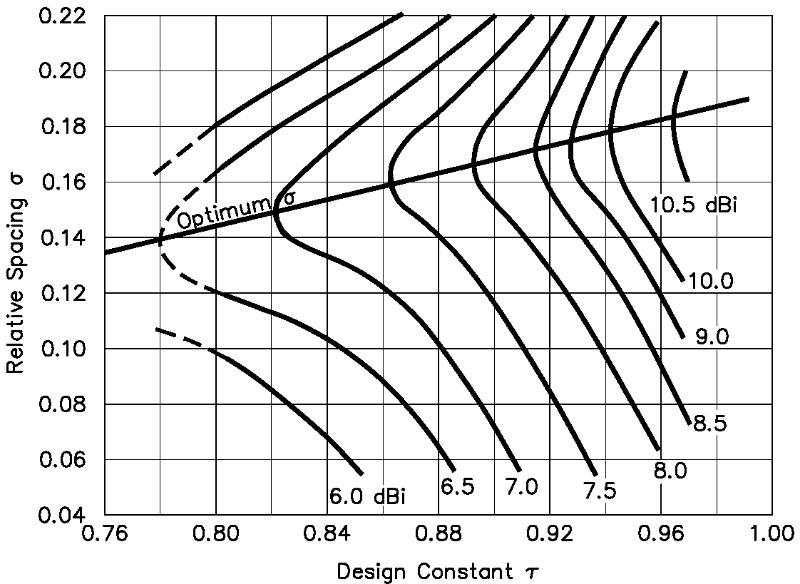
\includegraphics[width=1\textwidth]{figures/Yannis/Log_gain}
\caption{The parameters tau and sigma can be chosen from this graph. The line for optimum sigma is for those designers who want maximum gain\cite{balanis,Log}}
\label{log_gain}
\end{figure}

\begin{subequations}
\begin{align}
    a&=tan^{-1}[\frac{1-\tau}{4 \sigma}]=tan^{-1}[\frac{1-0.9}{4 \cdot 0.07}]=19.65^{\circ} \\
    B_{s}&=B \cdot B_{ar}=\frac{f_{high}}{f_{low}} (1.1+7.7(1-\tau)^2 \cdot cot(a))= \frac{400}{200} \cdot 1.316=2.631 \\
    N&=1+\frac{ln(B_{s})}{ln(\frac{1}{\tau})}=10.2 \approx 10 \ elements \\
    L&=\frac{c}{f_{low}} (1-\frac{1}{B_{s}}) \frac{cot(a)}{4}=0.6509 \ meters \\
    Z_{a}&=120(ln(\frac{l_{max}}{d})-2.25)=120 \cdot (ln(\frac{0.75}{0.019})-2.25)=171 \ \Omega
\end{align}
\label{eq: LPDA}
\end{subequations}

,where $l_{max}=\frac{c}{2 \cdot f_{min}}$ is the length of the maximum element and d=1.9 cm, which is the outer diameter of each element. Usually, a balun is needed in order to regulate the input impedance to desired values. 

LPDAs have a wide 3 dB beamwidth, which most of the times calculated through simulations, measurements or empirical tables. One f these tables is shown in figure \ref{hpbw_log}. Because of this wide beamwidth, LPDAs are not the best choice for our directional application, although if directivity is not our main concern there are manufacturers that sell very appealing, foldable antennas, some of them are presented in appendix \ref{LPDA1}. Finally, LPDAs are linear polarized, thus we have to mount two different, orthogonal antenna booms or one crossed design to receive properly the random polarization's orientation. Of course, this mean an extra 3 dB loss. A summary of the most suitable parameters of an LPDA for our mission can be found in table \ref{table: LPDA}.

\begin{figure}[htb]
\centering
    \captionsetup{width=0.8\textwidth}
        \centering
        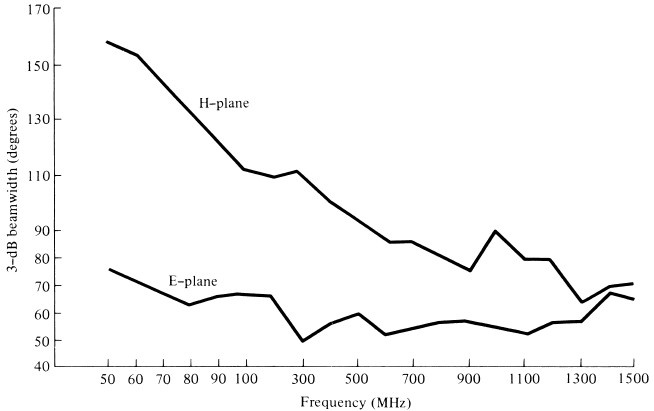
\includegraphics[width=1\textwidth]{figures/Yannis/HPBW_Log.jpg}
        \caption{Half power beamwidth for commercial log-periodic dipole arrays\cite{balanis}}
        \label{hpbw_log}
\end{figure}
\begin{figure}[htb]
\centering
        \captionsetup{width=0.8\textwidth}
        \centering
        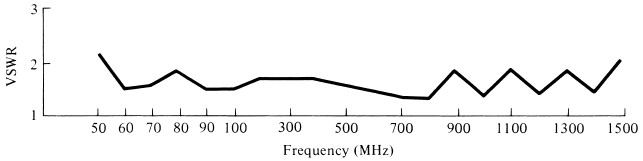
\includegraphics[width=1\linewidth]{figures/Yannis/VSWR_log.jpg}
        \caption{VSWR (Voltage Standing Wave Ratio) for commercial log-periodic dipole arrays\cite{balanis}}
        \label{vswr_lpda}
\end{figure}

\begin{table}[htb]
\begin{tabular}{| c | c | c | c | c | c | c | c |}
\hline
 $\tau$ & $\sigma$ & $f_{high}$ (MHz) & $f_{low}$ (MHz) & Gain (dBi) & HPBW & L (mm) & N \\ 
 \hline
 0.9 & 0.07 & 400 & 200 & 7 & (E)60$^\circ$-(H)100$^\circ$ & 650 & 10 \\
 \hline
\end{tabular}
\caption{Potential Log-Periodic Dipole Array design.}
\label{table: LPDA}
\end{table}

\paragraph{Helical Antennas Design}
Another type of antennas with a lot of potential in our mission is helical antenna. This antenna type is consisting of a conducting wire wound in the form of a helix, which in most cases is mounted over a ground plane. There are two modes that a helical antenna can operate and these are the normal mode and the axial. At normal mode the antenna resembles a monopole or dipole, so it has omnidirectional characteristics and linear polarization. We are interested in directional antennas, thus we will focus on the axial mode. The axial mode provides a directional antenna beam, radiating off the ends of the helix along the antenna's axis (end-fire). Moreover, the latter mode creates a circular polarized wave, which is mandatory for our application. A typical helical antenna with its radiation pattern is depicted in figure \ref{helical}.

\begin{figure}[htb!]
    \centering
    \captionsetup[subfigure]{width=0.45\textwidth}
    \subfloat[A typical representation of a helical antenna. The most important parameters, which determine its radiation pattern are shown\cite{helix}]{
        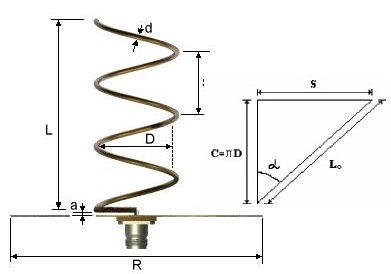
\includegraphics[width=.48\textwidth]{figures/Yannis/helix.jpg}
        \label{helix1}
    }
    \subfloat[Radiation pattern of helical antenna when operating in axial mode\cite{helix}]{
        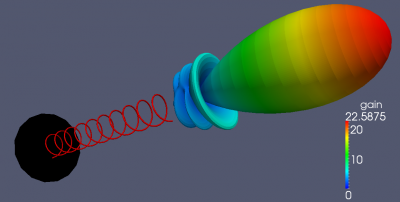
\includegraphics[width=.48\textwidth]{figures/Yannis/H2.png}
        \label{helix_pat}
    }
    \caption{Helical antenna sketch and radiation pattern.}\label{helical}
\end{figure}

The main constraints in building and using a helical antenna for our purposes would be again its total length, the beamwidth, the gain and the remaining distance to the ice layer. In order to examine the behaviour of such antennas the definition of the basic characteristics is needed. As it is shown in figure \ref{helix1} D represents antennas diameter, N turns of wire, d radius of wire and S the gap between turns. The overall length is $L=N \cdot S$ and the circumference of a single turn is $C=\pi \cdot D$. Last of the mechanical parameters are pitch angle of helix $a$ and R the reflector size, which must be at least 3/4 of the operating wavelength $\lambda$. In addition, we must take into account some experimentally derived guidelines, such as the value of pitch angle $a$ should be between $12^\circ$ and $14^\circ$. If $a$ is not in the specified range anomalies in the performance can occur. Also, the following formulas (eq. \ref{helical_eq}) are valid for $N \geq 3$ and $<3/4C/\lambda<4/3$ \cite{balanis2}.

For our design a trade off between total length and the parameters of frequency, C and S must be made. Generally, more turns (higher N) provide higher directivity $D_{0}$ and also the frequency dependence of the input impedance is smaller, but on the other hand the length can be disturbing big. For our mission we experimented with a MATLAB code (appendix \ref{matlab}) in different specifications and we ended up with the most suitable, as they presented in tables \ref{table: Helicals1} and \ref{table: Helicals2}. Additionally, we examined the possibility of using an array of helical antennas, but it can be seen for our frequencies it is more efficient (mainly gain-wise) to use in element. The following equations were used for this design \cite{balanis2}.

\begin{subequations}
\begin{align}
    &C=\pi \cdot D \\
    &a=tan^{-1}(\frac{S}{C}) \\
    &L=N \cdot S \\
    &R=\frac{3}{4} \lambda \\
    &Z_{in}=140 \cdot (\frac{C}{\lambda}) \\
    &HPBW=\frac{52 \cdot \lambda^{\frac{3}{2}}}{C \cdot \sqrt{N \cdot S}} \\
    &D_{0}=\frac{52 \cdot \lambda^{\frac{3}{2}}}{C \cdot \sqrt{N \cdot S}} \\
    &AR=\frac{2N+1}{2N} 
\end{align}
\label{helical_eq}
\end{subequations}

Except for a single helical antenna, we are simulated the behaviour of an array of helical antennas to examine if it is beneficial to use this implementation. The extra equations for an array are shown below (eq. \ref{helical_array}). Two approaches for the directivity were used, a simple one ($D_{array}$) and one taking into account the Hansen-Woodyard ($D_{HW}$) approximation. As it is presented in \ref{table: Helicals1} and \ref{table: Helicals2}, the array design it is not that useful for our frequencies, because in order to have better performance than the single helical antenna, more than 5 elements are needed.

\begin{subequations}
\begin{align}
    &dis=1.5 \cdot \lambda \\
    &D_{array}=N_{elem} \cdot (1+\frac{L}{dis})(\frac{dis}{\lambda}) \\
    &D_{HW}=1.805(N_{elem}(1+\frac{L}{dis})(\frac{dis}{\lambda})) 
\end{align}
\label{helical_array}
\end{subequations}
, where $N_{elem}$ is the number of array's elements and $dis$ is the distance between them. 

\begin{table}[htb]
\centering
\begin{tabular}{| c | c | c | c | c |}
\hline
 f (MHz) & Gain (dBi) & HPBW & Length (mm) & $Gain_{array}$ \\ 
 \hline
 300 & 7.8 & 64.5$^\circ$ & 800 & 16.6 \\  
 \hline
 340 & 23.6 & 37$^\circ$ & 1000 & 19\\
 \hline
  400 & 24.71 & 36.23$^\circ$ & 876 & 19.2 \\
 \hline
\end{tabular}
\caption{Helical antenna with 4 turns (N=4) specifications. The last column shows the values of gain in dBi for an array of 4 elements.}
\label{table: Helicals1}
\end{table}

\begin{table}[htb]
\centering
\begin{tabular}{| c | c | c | c | c |}
\hline
 f (MHz) & Gain (dBi) & HPBW & Length (mm) & $Gain_{array}$ \\ 
 \hline
 300 & 5.8 & 74.5$^\circ$ & 600 & 15.1 \\  
 \hline
 340 & 17.7 & 42.8$^\circ$ & 750 & 16.9\\
 \hline
  400 & 18.5 & 41.8$^\circ$ & 657 & 17.2 \\
 \hline
\end{tabular}
\caption{Helical antenna with 3 turns (N=3) specifications. The last column shows the values of gain in dBi for an array of 4 elements.}
\label{table: Helicals2}
\end{table}
A more detailed table for helical antennas can be found in appendix \ref{table: Helicals}.

As it is shown from tables \ref{table: Helicals1} and \ref{table: Helicals2}, the most suitable case is in frequency 340 MHz, where the total length of the antenna is 750 mm, the maximum gain is 17.7 dBi and the half power beamwidth is 42.8$^\circ$. There is also 250 mm free space between the end of the antenna and the ice, which could be enough to ignore ice as a near field obstacle. The gain exceeds our expectation, but bibliography states that these values may be exaggerated. But even in these case, the gain is still more than enough and helical antennas can receive or transmit circular polarization without the need of any modifications or additional losses. So, up to now it seems that a helical antenna is the most appealing option.

\paragraph{Parabolic Dish Design}
Parabolic dish antennas are very directional, high gain antennas, which are used mainly for the frequency range 2-15 GHz. For lower frequencies, like ours, the dish diameter increases to several meters. The basic formulas, which describe a dish antenna behaviour are presented below (eq. \ref{dish_eq}).

\begin{subequations}
\begin{align}
    &G=10 \cdot log_{10}(k \cdot (\pi \frac{D}{\lambda})^2) \\
    &HPBW=60 \cdot \frac{\lambda}{D}
\end{align}
\label{dish_eq}
\end{subequations}

\begin{table}[htb]
\centering
\begin{tabular}{| c | c | c | c | c |}
\hline
 f (MHz) & Gain (dBi) & HPBW & Diameter (mm) & k \\ 
 \hline
 300 & 7.2 & 66.6$^\circ$ & 900 & 0.66 \\  
 \hline
 340 & 8.3 & 58.8$^\circ$ & 900 & 0.66\\
 \hline
  400 & 9.7 & 50$^\circ$ & 900 & 0.66\\
 \hline
\end{tabular}
\caption{Parabolic antenna's specification for different frequencies.}
\label{table: dish}
\end{table}

, where G is the gain in dBi, D is the diameter of the parabolic reflector in metres and k is the efficiency factor which is generally around 50\% to 70\%. The parabolic reflector antenna gain efficiency is dependent upon a variety of factors, which are all multiplied together to give the overall efficiency. These factors are radiation efficiency, aperture taper efficiency, spillover efficiency, surface error, cross polarization, etc. The design of a parabolic antenna is way more complex, so in order to achieve very good results optimization of the feed point and a choice between different type of dish implementations must take place. By different type of dish implementations is meant, the Cassegrain, Gregorian or off-axis design. In the context of this section, we will not go any further because as it is clear from the results shown in table \ref{table: dish}, a parabolic antenna in this frequency range and under the restriction in diameter can not be really directional. Although, the gain levels are sufficient if we would like to go with a more wide HPBW.  



\subsubsection{Microstrip Antenna Array}
%\paragraph{Microstrip Antenna Array}
\label{microstrip antenna}

Another very famous antenna type is microstrip antennas or patch antennas. This type of antennas are low profile, conformable to planar and non-planar surfaces, simple and inexpensive to manufacture using modern printed-circuit technology. They are also mechanically robust when mounted o rigid surfaces, compatible with MMIC designs and when the particular patch shape and mode are selected they are very versatile in terms of frequency, polarization, pattern and impedance. Moreover, by using adaptive elements multiple resonant frequencies, impedances, polarizations and patterns can be achieved. Major operational disadvantages of microstrip antennas are their low efficiency, low power, high Q (quality factor), poor polarization purity and very narrow, which is typically only a fraction of few percent. In our range of frequencies, 300-400 MHz, patch antennas can be quite large with respect to other applications and frequencies. As it is clear the major reason why to use these antennas is the compactness they offer to our mission. If we can live with their disadvantages then is a fairly good alternative. 

As it happens very often, we use patch antennas in antenna arrays in order to increase their directivity and gain. This can be done also here wherever is this possible. Typically, the radiation of a single patch antenna is not very suitable for a high loss link so the array design is one-way road. Patches transmit in circular polarization if this is necessary with fairly low complexity. Also, circular patches can be designed if this is necessary. 

The modeling of a patch antenna is quite laborious and demands high end software. At this report the fundamental calculations of the dimensions of the antenna have been made without the use of any sophisticated antenna software, but using closed form equations, which can be found in \cite{balanis} chapter 14. The approach it is used called transmission line model and it can model antenna's behaviour acceptably well. After the determination of the desired dimension's an expansion will take place in order to use patch antennas in an array.
The characteristics of a rectangular microstrip antenna depends mainly on its substrate's dielectric coefficient ($\epsilon_{r}$), its length (L), width (W) and substrate height (h). The choice of $\epsilon_{r}$ should be done judiciously, because the decrease of it corresponds in higher efficiency and larger bandwidth, but larger dimensions. The height h has the opposite behaviour. The following equations (\ref{patch_eq}) were used to find the dimensions of the antenna when the excitation source are in the $TM_{010}$ dominant mode. Once we know the resonant frequency, the dielectric constant of the material we use for substrate and its height we define $\epsilon_{eff}$, W and L.
\begin{subequations}
\begin{align}
   &W=\frac{c}{2f} \sqrt{\frac{2}{\epsilon_{r}+1}} \\
   &\epsilon_{eff}=\frac{\epsilon_{r}+1}{2}+\frac{\epsilon_{r}-1}{2}[1+12\frac{h}{W}]^{-1/2} \\
   &\Delta L=0.412 h \frac{(\epsilon_{eff}+0.3)(\frac{W}{h}+0.264)}{(\epsilon_{eff}-0.258)(\frac{W}{h}+0.8)} \\
   &L_{eff}=\frac{\lambda}{2}+2\Delta L
\end{align}
\label{patch_eq}
\end{subequations}
, where c is light's speed, $\Delta L$ is length's increase because of $\epsilon_{eff}$.

Solving the above equations for different substrates, as seen in figure (\ref{substrate}), height $h=0.0589 \lambda$ we find the following dimensions.

\begin{figure}[ht]
\centering
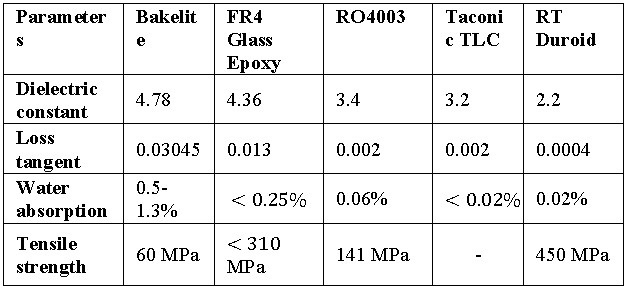
\includegraphics[width=.75\textwidth]{figures/Yannis/substrate.jpg}
\caption{Properties of different substrates. \cite{substrates}}
\label{substrate}
\end{figure}

\begin{table}[ht]
\centering
\begin{tabular}[width=.75\textwidth]{| c | c | c | c | c | c |}
\hline
 - & \textbf{Bakelite} & \textbf{FR4 Glass Epoxy} & \textbf{RO4003} & \textbf{Taconic TLC} & \textbf{RT Duroid} \\ 
 \hline
 \textbf{$\epsilon_{r}$} & 4.78 & 4.36 & 3.4 & 3.2 & 2.2 \\  
 \hline
 \textbf{L (mm)} & 290.9 & 305.2 & 336.9 & 344.8 & 395 \\
 \hline
 \textbf{W (mm)} & 202.7 & 215.3 & 244.2 & 251.7 & 301.8 \\
 \hline
\end{tabular}
\caption{Patch antenna's dimensions for different dielectric constant $\epsilon_{r}$. f=300 MHz}
\label{table: subs300}
\end{table}

\begin{table}[ht]
\centering
\begin{tabular}[width=.75\textwidth]{| c | c | c | c | c | c |}
\hline
 - & \textbf{Bakelite} & \textbf{FR4 Glass Epoxy} & \textbf{RO4003} & \textbf{Taconic TLC} & \textbf{RT Duroid} \\ 
 \hline
 \textbf{$\epsilon_{r}$} & 4.78 & 4.36 & 3.4 & 3.2 & 2.2 \\  
 \hline
 \textbf{L (mm)} & 216.4 & 228.9 & 252.7 & 258.6 & 269.3 \\
 \hline
 \textbf{W (mm)} & 150.3 & 161.3 & 183 & 188.6 & 226.1 \\
 \hline
\end{tabular}
\caption{Patch antenna's dimensions for different dielectric constant $\epsilon_{r}$. f=400 MHz}
\label{table: subs400}
\end{table}

Knowing from antenna theory that the radiating slots of a patch antenna can be seen as two independable dipoles, we can use this approximation to find the gain using the array factor (AF). If we assume a assume a dielectric constant, which compromise size and efficiency, we can choose the RO4003 from \ref{table: subs300} or \ref{table: subs400}. Thus, if the area below our lander vehicle is 1 $m^2$ we can design a 6 element patch array antenna with element's size 377x244 mm if we are go for the lower frequency of 300 MHz. According to Balanis' approximated formulas we can have directivity for each slot equal to 4 dB and around 5.8 dB for the whole antenna (two slots). In order to increase the directivity using the array design of 6 elements we can achieve a half power beamwidth about $40^{\circ}$, as it can be seen in figure (\ref{array}). In case we design the antenna for 400 MHz, the patch size will be smaller, thus more antennas can be placed to the available space. Always we have to consider that higher frequencies correspond to higher losses and in case of patch antennas without any substantial increase in gain and beamwidth.

\begin{figure}[ht]
\centering
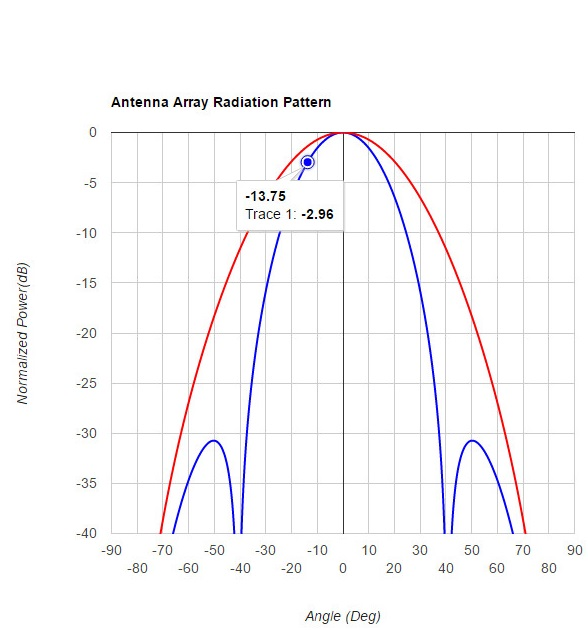
\includegraphics[width=.75\textwidth]{figures/Yannis/2results.jpg}
\caption{Half power beamwidth for an antenna array of 6 microstrip antennas (red curve) and for an antenna array of 12 microstrip antennas (blue curve). Both are pointing at broadside.}
\label{array}
\end{figure}

Finally, in order to determine the the gain we have to know the radiating efficiency. As it has stated, taking into account the absence of the necessary dedicated software for antenna analysis, such as HFSS and CST, we are trusted the results from \cite{substrates} as they are shown in figure (\ref{array result}). The last step is to find the gain of the antenna. The designing characteristics of the aforementioned antenna of 6 elements are summing up in table (\ref{table: results}).

\begin{figure}[ht]
\centering
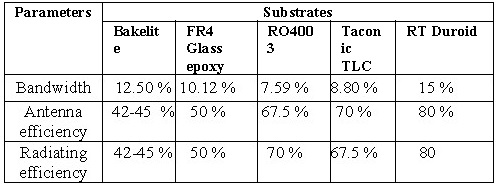
\includegraphics[width=.75\textwidth]{figures/Yannis/results.jpg}
\caption{Fractional bandwidth, antenna efficiency and radiating efficiency for a single patch antenna. The measurements reported in \cite{substrates} correspond to frequency 10 GHz, although due to poor dependence of these quantities from frequency we can use them for our approximations.}
\label{array result}
\end{figure}

\begin{table}[ht]
\centering
\begin{tabular}{| c | c | c | c | c | c | c | c |}
\hline
 \textbf{f (MHz)} & \textbf{$\epsilon_{r}$} & \textbf{W (mm)} & \textbf{L (mm)} & \textbf{D (dB)} & \textbf{$\epsilon_{rad}$} & \textbf{G (dB)} & FBW \\ 
 \hline
 300 & 3.4 & 244 & 337 & 5.76 & 70 \% & 4.03 & 7.59 \% \\
 \hline
 400 & 3.4 & 183 & 252 & 9.4 & 70 \% & 6.58 & 7.59 \% \\
 \hline
\end{tabular}
\caption{Design characteristics for a patch antenna array. 300 MHz corresponds to 6 elements array and 400 MHz to 12 elements. D stands for maximum directivity and G for maximum gain.}
\label{table: results}
\end{table}

An important part of microstrip antennas (and especially in arrays) is the input impedance and matching. The input admittance of a slot and thus for a patch antenna is given by using Huygens's equivalent principle. The procedure is quite laborious and will not be shown here. Although, a useful consequence is that we can match the input admittance by a very easy technique, using a small inset in each individual patch. Also, if circular polarization is needed many different techniques of feeding can be used. Of course, since we are talking for an array antenna, the appropriate phase differences should be introduced between the array elements. About feeding we can use either uniform or nonuniform antennas, which mean constant or varying magnitude of the elements. Non-uniform arrays are more preferable since they present lower sidelobe and grating lobe levels, but on the other hand worst directivity. Good cases for non-uniform amplitude coefficients are the binomial and Tschebysheff's polynomial. 

\subsection{Penetrator Antenna}

As it was mentioned in \ref{microstrip antenna}, the great advantage of patch antennas are their compact size. Having in mind the extremely limited available space at penetration vessel to place an antenna, the option of a patch antenna or a small array of them seems a good alternative. The analysis is exactly the same as it was done previously, so only minor modifications are necessary. First of all, array's elements must be placed on the sides of the vessel due to limited area on the top. Moreover, the antenna design must be an end-fire, which means that the antenna beam points along the axis where the elements are placed, thus the desired beam will point at $\theta=0$. In order to achieve that properly phase difference should be introduced to the elements. The positive side of that is the possibility of redirecting the beam in case of misalignment between penetrating vessel and lander vehicle antenna. Taking into account the size of the vessel, approximately 10-15 cm outer diameter, the patch antennas should be placed around its periphery. 

\begin{table}[ht]
\centering
\begin{tabular}{| c | c | c | c | c | c | c | c |}
\hline
 \textbf{f (MHz)} & \textbf{$\epsilon_{r}$} & \textbf{W (mm)} & \textbf{L (mm)} & \textbf{D (dB)} & \textbf{$\epsilon_{rad}$} & \textbf{G (dB)} & FBW \\ 
 \hline
 300 & 3.4 & 244 & 337 & 4.45 & 70 \% & 3.12 & 7.59 \% \\
 \hline
 400 & 3.4 & 183 & 252 & 7.12 & 70 \% & 4.86 & 7.59 \% \\
 \hline
\end{tabular}
\caption{Design characteristics for a patch antenna array of penetrator vessel. 300 MHz corresponds to 3 elements array and 400 MHz to 5 elements. D stands for maximum directivity and G for maximum gain.}
\label{table: results_pen}
\end{table}

\subsection{Link Budget Analysis}

The link budget will take place in this section, in order to assess which one of the above configurations is most suitable for our application. In this part we are interested in high directional link with the best possible efficiency and lower possible size, taking into account the ice losses with relation to frequency. Moreover, the necessary data rate should be kept in mind. As it has mentioned above, the period of the orbiter around Europa is approximately 13 days, which means penetrator vessel sends data to the lander vehicle during this period and the latter stored there, until the next pass of the orbiter. The available time, when line of sight between ground and space segment will have been established longs only few hours (around 3 hours), thus we have to deliver any stored data from 13 days in this small interval. This is our main driver concerning data rates and it limits the uploaded data size to 1 Gbit (giga bit) in three hours. Consequently, we can calculate the necessary data rate between penetrator-orbiter should be 1 Kbps (kilo bit per second) to achieve 1 Gb accumulation in 13 days. Although, if demand for higher data rates occurs, we can push the limits of our equipment compromising the signal to noise ratio.

The following link budget calculations are based on Friis formula of propagation, taking into account propagation losses due to the distance (distance in worst case scenario is 10 Km), losses due to ice, as described in \ref{losses}, losses from different components (transmission lines, tranceivers, etc.) and polarization mismatches. Due to indeterministic nature of ice losses, two average estimation will be included in the calculations. The first will be an estimated worst case scenario with ice losses of 8 dB/Km and an intermediate case scenario with 6 dB/Km. Finally, for each different antenna design, the link budget with a 1 dB required $E_{b}/N_{0}$ will be found and then an overall estimation will take place. 

\begin{table}[ht]
\centering
\begin{tabular}{| c | c | c | c | c | c |}
\hline
 \textbf{Ant. Type} & \textbf{$G_{Tx}$ } & \textbf{$G_{Rx}$ } & \textbf{Add. Losses } & \textbf{Pol. Losses} & $E_{b}/N_{0} $ \\ 
 \hline
 Crossed-Yagi & 8.6 dB & 3.12 dB & 0.5 dB & 3 dB & 5.4 dB \\
 \hline
 LPDA & 7 dB & 3.12 dB & 0.5 dB & 3 dB & 3.8 dB\\
 \hline
 Helical & 7.8 dB & 3.12 dB & 0.5 dB & 0 dB & 7.6 dB\\
 \hline
 Parabolic & 7.2 dB & 3.12 dB & 0.5 dB & 0 dB & 7 dB\\
 \hline
 Microstrip & 4 dB & 3.12 dB & 0.5 dB & 0 dB & 3.8 dB\\
 \hline
\end{tabular}
\caption{Link budget analysis for the different types of antennas, at frequency of 300 MHz, for the worst case scenario attenuation due to ice losses (8 dB/km). The computations take into account the dielectric constant of the ice, bit rate of 1 Kbps and transmitted power of 10 Watts. The distance which is calculated is 10 km of ice with impurities.}
\label{table: link_budget}
\end{table}

\subsubsection{Link Budget Analysis \& Feasibility Assessment}
\paragraph{Yagi \& LPDA antennas}
Table \ref{table: link_budget} is a link budget analysis which concentrates on telecommunication characteristics. Beside them we have to take into account also dimensions and the corresponding beamwidth in any case to find out the most suitable antenna, the number of elements/turns, array factor, etc. As mentioned earlier, Yagi and LPDA antennas are quite efficient, but on the other hand they take more space because of the necessary distance between the elements and need a sufficient distance from the first "obstacle" in the near field, ice in our case. Moreover, there is an extra 3 dB loss, due to polarization mismatches in order to be able to receive/transmit circular polarization. These reasons are enough to not consider Yagis and LPDAs as our first priority. 
\paragraph{Helical antennas}
Helical antennas are quite promising not only because of their very good gain and efficiency, but also for their extremely good beamwidth in this frequency range. Another advantage of them is the ability to built a planar array, with small footprint, in order to increase the gain and decrease the beamwidth. Finally, we can manipulate each element independently, which provides more freedom to our design. After the above, we can see from  tables \ref{table: Helicals1} and \ref{table: Helicals2} that there are substantial differences between the frequencies and the use of an array of helical antennas. Having in mind the strict limitation of space under our lander vehicle, the most suitable helical antenna is around 340 MHz and N=3 (table \ref{table: Helicals2}). This specific design is a compromise between long antennas, high gain, sufficient beamwidth to consider the antenna directional and fairly low frequency to avoid high ice losses. It is also noticeable that the single element exceeds the performance of an array, which is not strange in these frequencies. We could choose also the respective antenna at 400 MHz, but the increase of ice losses at 400 MHz are far higher than the almost 1 dB extra gain. Last but not least, this design has the advantage that can be folded and unfolded easily. We can have the coil compressed and attached to a wire, in order to provide the necessary tension to keep it folded. When we want to deploy the antenna we will need only a resistor and a very small current to produce some heat and melt the wire, thus our antenna will be deployed as a reaction.
\paragraph{Parabolic/Dish antennas}
Parabolic antennas can approach very good efficiencies and provide the necessary gain. Their diameter and shape can fit below our vehicle, although it will be more difficult to fold and unfold this design comparing with helical antennas. Additionally, as it can be seen (table \ref{table: dish}) the beamwidth at the same frequencies as helicals, is much wider, thus these antennas are less directive. The above mentioned reasons are sufficient to exclude this design. 
\paragraph{Microstrip Antennas}
Microstrip antennas are well suited when space is high priority with the expense of low quality and small gain. Microstip antennas at 300 MHz present a gain only 4 dB, which cannot be compared with the other designs. Although, their inefficiency can be overlooked in the case of the penetrator vessel where the absence of space does not leave any other option.

Finally, the link budget for the proposed antenna (helical), in the frequency of 340 MHz and with N=3 is shown in table \ref{table:link_budget_helix}.

\begin{table}[ht]
\centering
\begin{tabular}{| c | c | c | c | c | c |}
\hline
 \textbf{Ant. Type} & \textbf{$G_{Tx}$} & \textbf{$G_{Rx}$} & \textbf{Add. Losses} & \textbf{Pol. Losses} & \textbf{$E_{b}/N_{0}$} \\ 
 \hline
 Helical & 17.7 dB & 3.12 dB & 0.5 dB & 0 dB & 17.5 dB \\
 \hline
\end{tabular}
\caption{Link budget analysis for a helical antenna, at frequency of 340 MHz, for the worst case scenario attenuation due to ice losses (8 dB/km). The computations take into account the dielectric constant of the ice, bit rate of 1 Kbps and transmitted power of 10 Watts. The distance which is calculated is 10 km of ice with impurities.}
\label{table:link_budget_helix}
\end{table}

\subsection{Implementation's hazards}
As discussed in this section, directivity is a desirable characteristic of antennas when you want to concentrate the beam in a specific direction. Nevertheless, in some cases high directivity can lead to mission failure, especially when the "target" object changes direction rapidly. In our application this is not the case, but misalignments can occur because of different unexpected factors. For instance, while the penetrator will be melting the ice, the heat may not propagating isotropically, thus gradually the penetrator will start diverging from the expected route. If we do not foresee the capability of beam steering and the deviation become large, there is possibility to lose the penetrator vessel from our "field of view". In other cases, may will be desirable to change the route of our penetrator to avoid obstacles, such as rocks, liquid pools, etc. In either cases, we must have the possibility to steer the beam or change its beamwidth in such manner to retain the communication.

Another problem which is possible to come across is the landing on a steep slope, instead of a relative smooth area. In the former case, we must built the antenna under the lander vehicle in order to be able to point at different directions and not only perpendicular to vehicle's surface, as shown in figure \ref{ant steer}. This can be done by placing the antenna onto a steerable ground plane or by steering only the antenna's coil without moving the ground plane. The latter case will result in a slightly squinted beam with respect to the normal unit vector of ground plane, but if we know the desired direction we can compensate for this misalignment, in order to achieve the maximum directivity.

\begin{figure}[ht]
\centering
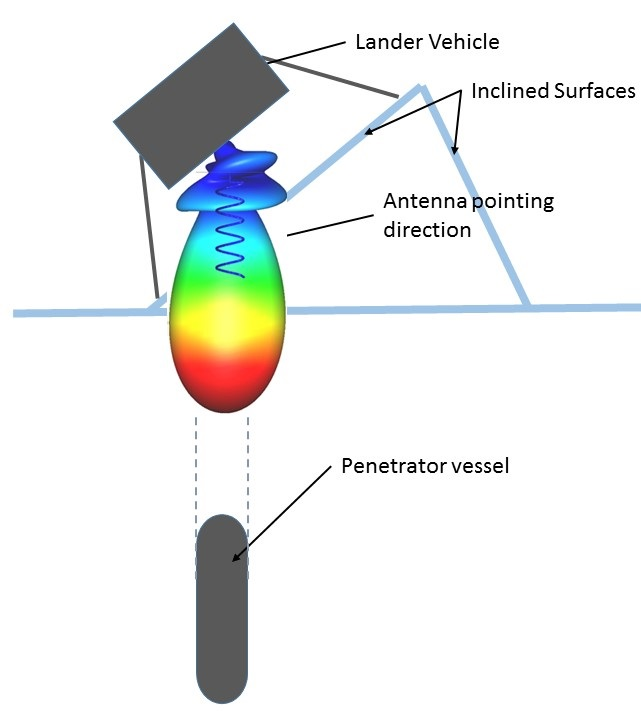
\includegraphics[width=.6\textwidth]{figures/Yannis/normal.jpg}
\caption{The antenna beam must point at penetrator vessel, even if the landing take place at an inclined surface.}
\label{ant steer}
\end{figure}


% LD Link
\autsubsection{Low Directivity Link}{Gustavo Feijóo Carrillo}
\begin{figure}[htb]
	\centering
	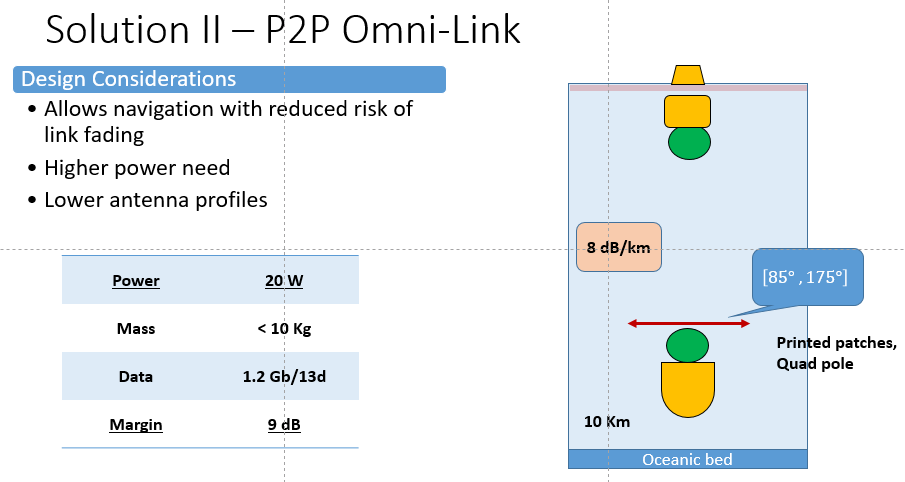
\includegraphics[width=\textwidth]{figures/comms/iceLink-p2p-LowD}
	\caption{ \textit{DRAFT} Sol II.}
	\label{fig:iceLink-p2p-LowD}
\end{figure}

% Ice embedded relays
\subsection{Relay Link}
\begin{figure}[htb]
	\centering
	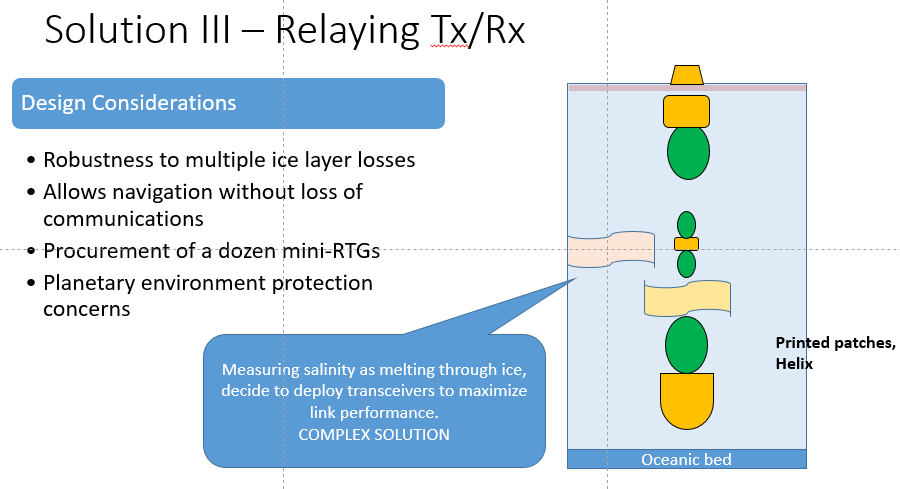
\includegraphics[width=\textwidth]{figures/comms/iceLink-relay}
	\caption{ \textit{DRAFT} Sol III relays.}
	\label{fig:iceLink-relay}
\end{figure}
	

\section{Probe-to-Penetrator}

%\subsection{High Directional Link}

\autsection{Highly Directional Link}{Nissopoulos Ioannis}

\subsection{Link Description}

\paragraph{Directional antennas}
Directivity is a fundamental antenna parameter, which measures how much power radiated or received in a specific direction from the antenna. A directional antenna is the exact opposite of an omni-directional antenna, which transmits or receives equally from all directions. Directional antennas provide increased performance and reduced interference from unwanted sources, because of their construction and their basic principles. Well known applications for high directional antennas are among others NASA's Deep Space Network (DSN), terrestrial communication links, such as satellite television and cellular repeaters, where high position accuracy and propagation in long distances are needed. In general, high directional antennas are used in every application where high data rates, high gain and reduced interference is mandatory.

The main principle of directional antennas is their ability to concentrate almost all the transmitted power to small beamwidths, instead of illuminating wider solid angles. Saying that, they do not sacrifice any power to unwanted directions, but achieve high gain (more than 10 dBi) for specific solid angles. On the other hand, high directional antennas can reach their targets only through very narrow beamwidths, which can be a significant bottle neck in many applications and especially when tracking in long distances is required. 

Typical types of directional antennas are parabolic antennas, helical antennas, yagi antennas, horn antennas, phased arrays, etc. Directivity and gain of such types of antennas can be affected from many different parameters, regarding their type and application. The number of elements and their spacing, their physical or synthetic aperture, their surrounding environment and the manufacturing material are some of the major criterion that can change the performance of a highly directive antenna considerably. 

\paragraph{Solution description}
In this subsection we will examine if it is possible to use a high directional link for the communication segment between the lander vehicle and the penetrator of our mission. The advantages and disadvantages will be analyzed thoroughly and finally an assessment of this possibility will take place. 

The aforementioned idea is based on a pair of highly directive antennas, which can be used to achieve high rates of data streams and a stable communication channel. One antenna will be installed on lander vehicle's bottom surface looking downwards, while the other one will be placed on the top surface of the penetrator facing upwards, towards the first antenna. The line of sight between these two antennas must always be free of obstacles and we must assure that the beamwidths of the antennas are aligned and cross each other all the time. \textbf{pic} Different types of antennas will be examined in order to find out which one them is the most efficient for the requirements of our mission.

\paragraph{Drivers of Comm Link}
The design of a communication link in an inhospitable environment as Europa's subsurface can be proved especial demanding and difficult, but definitely will not be our only limitation. Space and power consumption is most of the times the number one drivers in all remotely controlled missions. The first priority when an engineer designs a communication link is the selection of the frequency range for the specific mission. In order to do so, engineers have to take into account a lot of factors such as the host environment and the attenuation that implies, the desired bandwidth, the amount of data with the corresponding data rates, etc. 

As we expect, Europa's subsurface consists of several kilometers of ice, which is a factor that limits our choice of frequency range. As described in subsection \ref{sec:ice_losses}, the longer the wavelength we use the better penetration through the ice crust we can achieve. In other words, as we go down in frequency our losses due to ice layers are diminished. Longer wavelengths are also more effective against attenuation due to impurities, because the dimensions of these impurities particles (sulfates, debris rocks, etc.) expected to be in order of millimeters. Nonetheless, the frequency of an antenna is always bonded to its size, by means that lower frequencies correspond to bigger size of antennas. Having in mind our requirements for high directivity, gain and satisfying bandwidth we must keep the size of our antenna reasonable. Other parameters that affect this size can be the type of the antenna. Moreover, due to the limited available space we will provide ways to fold and deploy the antennas wherever it is necessary.  

% \textbf{Obstacles in the near field}

\subsection{Implementation}
In this paragraph, we will examine different type of antennas for the lander vehicle, but also for the penetrating vessel. The main criteria for choosing an antenna type are the size and the ease of folding and deployment, the providing gain and the beamwidth or directivity of the antenna. Other characteristics under examination will be the capability of steering, mechanically or electronically, and the achievable data rates. After the determination of the above, we will perform the link budget analysis for the specified link. 

At first, we will concentrate only on the lander vehicle's antenna and in the next part on penetrator's. In figure \ref{fig:J_spec} can be seen the highest frequency, which is free of Jupiter's radio emissions and it is around 50 MHz, thus this is the lowest frequency choice we can make. The wavelength of this frequency is approximately 6 meters, which is way bigger than 1 meter which is the estimated available space we have under the "belly" of our land vehicle. In order to overcome this problem, we will investigate the case of a slightly higher frequencies, above 150 MHz. 

Firstly, we will present the candidate types of antennas, which will be mounted beneath our lander vehicle. It is difficult to analyze all the different types of directional antennas in the context of this report, thus we will examine three major antenna's "families", which fulfill the requirements discussed above. The first antenna type is Yagi-Uda (or Yagi) antennas together with the log periodic dipole array (LPDA). The former are used mainly from radio amateurs and they are inexpensive but quite efficient antennas for lower frequencies. A distinctive characteristic of Yagi antennas is that their design and construction based most of the times in experimental measurements hands-on experience, rather than well documented formulas and heavy mathematics. Many radio amateurs share their experience and design characteristics in order to improve the basic design as Shintaro Uda and Hidetsugu Yagi had designed in 1962. The later are a special type of antennas, which are quite similar in design with Yagis, although their distinctive characteristic is the very broad bandwidth. Because of this LPDAs are used in UHF terrestrial TV, HF communications, EMC measurements etc.

\paragraph{Yagi-Uda Design}
Yagi-Uda antennas consist of a single driven element connected to the transmitter or receiver and additional parasitic elements. The parasitic elements operate by re-radiating their signals in a slightly different phase in relation to the driven element. In this way the signal is reinforced in some directions and cancelled out in others, so a high directivity is achieved. The length and the spacing of each parasitic element determined by the operational frequency, as well as the total length of the antenna. As it can be seen in figure \ref{Yagi}, a Yagi antenna is linear polarized, parallel to its elements dimension. This is a significant drawback of this design in case the user needs to exploit different polarizations. The solution to this can be the "crossed" Yagi-Uda antenna, which practically is two antennas with two orthogonal polarizations on the same boom. Crossed Yagis provide the capability to receive or transmit in circular polarization with a -3 dB trade off of your signal. If we finally will choose this antenna type for sure we need to consider the crossed version, because the received polarization will have been rotated randomly from the ice crust. LPDAs may look similar to Yagis, although their main principle is quite different. They consist of a number of dipole elements as well, but not all antenna elements are active at any given frequency. In other words, we can imagine a LPDA as an array of dipoles tuned in different frequencies and this is the reason why these antennas hold bandwidth more than few GHz. Another difference is that the main beam of this antenna comes from the "shorter" front. LPDAs used because of their wide bandwidth and not so much because of their gain or their bandwidth. For our purposes, this antenna type will not present so many attractive points, so we will not cover them thoroughly. 

\begin{figure}[htb]
    \centering
    \captionsetup[subfigure]{width=0.45\textwidth}
    \subfloat[A typical Yagi-Uda antenna with 3 directors, 1 driven element and 1 reflectors]{
        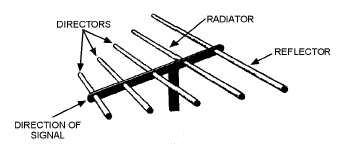
\includegraphics[width=.48\textwidth]{figures/Yannis/yagi.jpg}
        \label{Yagi}
    }
    \subfloat[The basic components of a log periodic dipole array. The forward direction is to the left in this sketch]{
        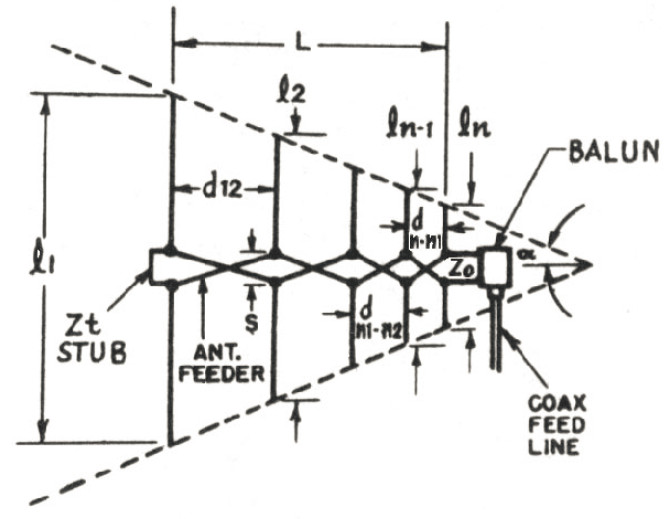
\includegraphics[width=.48\textwidth]{figures/Yannis/log2.jpg}
        \label{log}
    }
    \caption{}
\end{figure}

As it is mentioned above, the design of a Yagi-Uda antenna is usually approached with an optimization algorithm based on already existed designs. Mentioning that, the free software "Yagi Calculator" (from VK5DJ radio amateur, \url{http://www.vk5dj.com/yagi.html}) was used, which simulates the antenna and has as an output its gain, beamwidth, antenna length, etc. Our major bottleneck using Yagis will be first of all their boom length. According to many designs, the boom length should be at least 2.2 $\lambda$ in order to achieve the best performance out of the antenna. Our available space is approximately 1 meter, thus our antenna boom should be less than one meter, which corresponds practically to frequencies higher than 600 MHz. As it is clear, frequencies higher than 400 MHz present excessive losses and is impossible to be used for our application. Although, we can decrease boom length according to our desires with a trade off in gain and beamwidth. Another issue that we must take into account is the really close distant of ice from the tip of our antenna. This mean that the ice will be inside the near field of our antenna, which can causes serious troubles to our design. The limit between near and far field is given by Fraunhofer's formula $d=\frac{2D^2}{\lambda}$, where D is the largest dimension of the radiator and $\lambda$ is the wavelength of the radio wave. So, we conclude that in order to eliminate or at least reduce the effect of the near field because of the ice, we have to leave a distance equals d before the ice layer. Usually, this distance is very close to the boom length, thus we could claim that we need d=80\% of boom's length, in best case scenario. 

Having the length's limitation in mind the following results came up from the software.
\begin{table}[htb]
\begin{tabular}{| c | c | c | c | c |}
\hline
 f (MHz) & Gain (dBi) & Beamwidth (-3 dB) & Boom Length (mm) & Director No. \\ 
 \hline
 300 & 8.6 & 75 & 515 & 2 \\  
 \hline
 400 & 12 & 65 & 562 & 3\\
 \hline
  430 & 11 & 57 & 700 & 4 \\
 \hline
\end{tabular}
\caption{Potential Yagi designs for different frequencies.}
\label{table: Yagi}
\end{table}

It is shown from table \ref{table: Yagi} that the beamwidths, even at 430 MHz, are fairly wide and it is difficult to define an antenna with this values as absolutely directional. Moreover, in case of a crossed design the power divided into two radiating dipoles, so we have to substract 3 dB from each case.

\paragraph{LPDA Design}
In contrast, LPDAs can be operated over a range of frequencies and over this range its electrical characteristics gain, feed-point impedance, front-to-back ratio, etc. will remain more or less constant. The two most important parameters for LPDA are $\tau$ and $\sigma$, where $\tau$ is the ratio of the length of one element to its next longest neighbor and is constant for a given design for all elements and $\sigma$ is known as the “relative spacing constant” and along with $\tau$ determines the angle of the antenna’s apex, a. 

The design process starts choosing the desired gain in dBi and from \ref{log_gain} $\tau$ and $\sigma$ are determined. A good choice of gain for this type of antennas is around 7 dBi, which is also quite common in commercial applications. Having in mind that $\tau$ and $\sigma$ define the number of elements, thus the size of antenna's boom, we want to keep them at reasonable low numbers. Observing figure \ref{log_gain}, we choose $\tau=0.9$ and $\sigma0.07$ in order to have 7 dBi gain. Also, our operational bandwidth will be from 200 to 400 MHz.

In order to find out the total length of the antenna and its number of elements the apex angle must be calculated. The bandwidth for this design is computed afterwards and from this the number of elements N and the total length of the structure are computed. Finally, the average characteristic impedance of the elements $Z_{a}$ is calculated. In the next lines these calculations take place, according to \cite{balanis}, while the MATLAB code can be found in appendix \ref{matlab}.

\begin{figure}[htb]
\centering
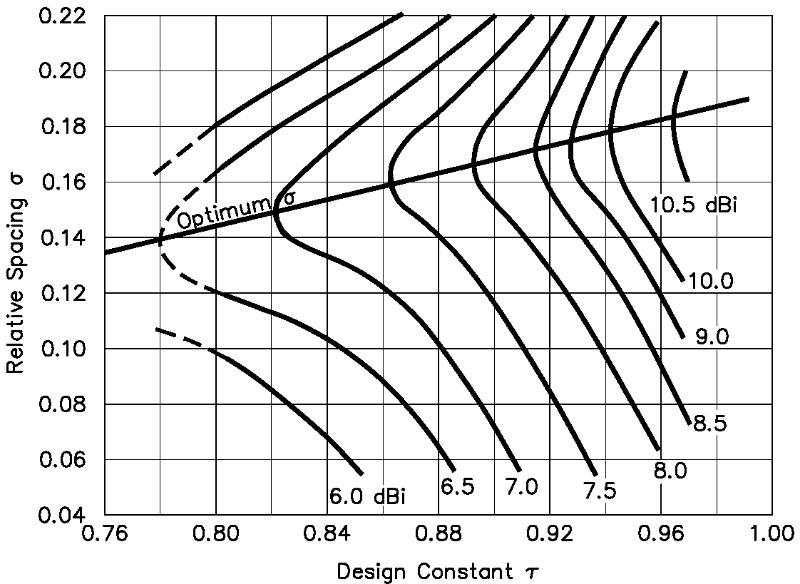
\includegraphics[width=1\textwidth]{figures/Yannis/Log_gain}
\caption{The parameters tau and sigma can be chosen from this graph. The line for optimum sigma is for those designers who want maximum gain\cite{balanis,Log}}
\label{log_gain}
\end{figure}

\begin{subequations}
\begin{align}
    a&=tan^{-1}[\frac{1-\tau}{4 \sigma}]=tan^{-1}[\frac{1-0.9}{4 \cdot 0.07}]=19.65^{\circ} \\
    B_{s}&=B \cdot B_{ar}=\frac{f_{high}}{f_{low}} (1.1+7.7(1-\tau)^2 \cdot cot(a))= \frac{400}{200} \cdot 1.316=2.631 \\
    N&=1+\frac{ln(B_{s})}{ln(\frac{1}{\tau})}=10.2 \approx 10 \ elements \\
    L&=\frac{c}{f_{low}} (1-\frac{1}{B_{s}}) \frac{cot(a)}{4}=0.6509 \ meters \\
    Z_{a}&=120(ln(\frac{l_{max}}{d})-2.25)=120 \cdot (ln(\frac{0.75}{0.019})-2.25)=171 \ \Omega
\end{align}
\label{eq: LPDA}
\end{subequations}

,where $l_{max}=\frac{c}{2 \cdot f_{min}}$ is the length of the maximum element and d=1.9 cm, which is the outer diameter of each element. Usually, a balun is needed in order to regulate the input impedance to desired values. 

LPDAs have a wide 3 dB beamwidth, which most of the times calculated through simulations, measurements or empirical tables. One f these tables is shown in figure \ref{hpbw_log}. Because of this wide beamwidth, LPDAs are not the best choice for our directional application, although if directivity is not our main concern there are manufacturers that sell very appealing, foldable antennas, some of them are presented in appendix \ref{LPDA1}. Finally, LPDAs are linear polarized, thus we have to mount two different, orthogonal antenna booms or one crossed design to receive properly the random polarization's orientation. Of course, this mean an extra 3 dB loss. A summary of the most suitable parameters of an LPDA for our mission can be found in table \ref{table: LPDA}.

\begin{figure}[htb]
\centering
    \captionsetup{width=0.8\textwidth}
        \centering
        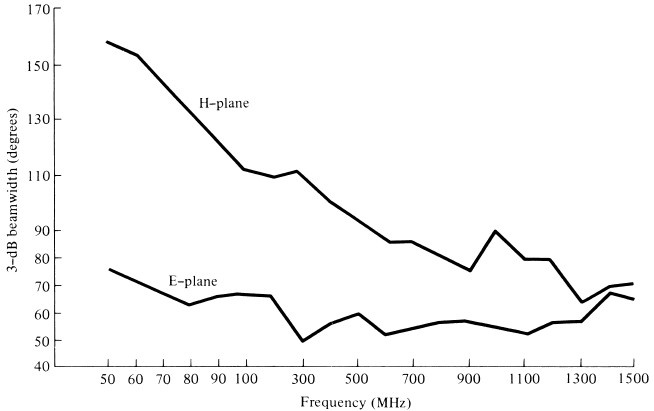
\includegraphics[width=1\textwidth]{figures/Yannis/HPBW_Log.jpg}
        \caption{Half power beamwidth for commercial log-periodic dipole arrays\cite{balanis}}
        \label{hpbw_log}
\end{figure}
\begin{figure}[htb]
\centering
        \captionsetup{width=0.8\textwidth}
        \centering
        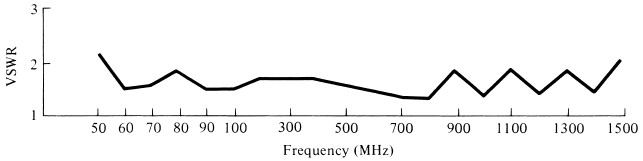
\includegraphics[width=1\linewidth]{figures/Yannis/VSWR_log.jpg}
        \caption{VSWR (Voltage Standing Wave Ratio) for commercial log-periodic dipole arrays\cite{balanis}}
        \label{vswr_lpda}
\end{figure}

\begin{table}[htb]
\begin{tabular}{| c | c | c | c | c | c | c | c |}
\hline
 $\tau$ & $\sigma$ & $f_{high}$ (MHz) & $f_{low}$ (MHz) & Gain (dBi) & HPBW & L (mm) & N \\ 
 \hline
 0.9 & 0.07 & 400 & 200 & 7 & (E)60$^\circ$-(H)100$^\circ$ & 650 & 10 \\
 \hline
\end{tabular}
\caption{Potential Log-Periodic Dipole Array design.}
\label{table: LPDA}
\end{table}

\paragraph{Helical Antennas Design}
Another type of antennas with a lot of potential in our mission is helical antenna. This antenna type is consisting of a conducting wire wound in the form of a helix, which in most cases is mounted over a ground plane. There are two modes that a helical antenna can operate and these are the normal mode and the axial. At normal mode the antenna resembles a monopole or dipole, so it has omnidirectional characteristics and linear polarization. We are interested in directional antennas, thus we will focus on the axial mode. The axial mode provides a directional antenna beam, radiating off the ends of the helix along the antenna's axis (end-fire). Moreover, the latter mode creates a circular polarized wave, which is mandatory for our application. A typical helical antenna with its radiation pattern is depicted in figure \ref{helical}.

\begin{figure}[htb!]
    \centering
    \captionsetup[subfigure]{width=0.45\textwidth}
    \subfloat[A typical representation of a helical antenna. The most important parameters, which determine its radiation pattern are shown\cite{helix}]{
        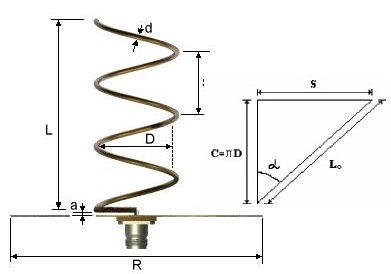
\includegraphics[width=.48\textwidth]{figures/Yannis/helix.jpg}
        \label{helix1}
    }
    \subfloat[Radiation pattern of helical antenna when operating in axial mode\cite{helix}]{
        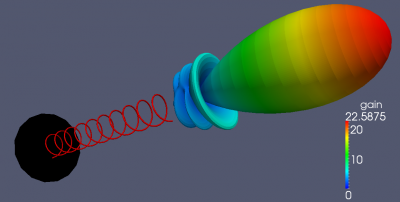
\includegraphics[width=.48\textwidth]{figures/Yannis/H2.png}
        \label{helix_pat}
    }
    \caption{Helical antenna sketch and radiation pattern.}\label{helical}
\end{figure}

The main constraints in building and using a helical antenna for our purposes would be again its total length, the beamwidth, the gain and the remaining distance to the ice layer. In order to examine the behaviour of such antennas the definition of the basic characteristics is needed. As it is shown in figure \ref{helix1} D represents antennas diameter, N turns of wire, d radius of wire and S the gap between turns. The overall length is $L=N \cdot S$ and the circumference of a single turn is $C=\pi \cdot D$. Last of the mechanical parameters are pitch angle of helix $a$ and R the reflector size, which must be at least 3/4 of the operating wavelength $\lambda$. In addition, we must take into account some experimentally derived guidelines, such as the value of pitch angle $a$ should be between $12^\circ$ and $14^\circ$. If $a$ is not in the specified range anomalies in the performance can occur. Also, the following formulas (eq. \ref{helical_eq}) are valid for $N \geq 3$ and $<3/4C/\lambda<4/3$ \cite{balanis2}.

For our design a trade off between total length and the parameters of frequency, C and S must be made. Generally, more turns (higher N) provide higher directivity $D_{0}$ and also the frequency dependence of the input impedance is smaller, but on the other hand the length can be disturbing big. For our mission we experimented with a MATLAB code (appendix \ref{matlab}) in different specifications and we ended up with the most suitable, as they presented in tables \ref{table: Helicals1} and \ref{table: Helicals2}. Additionally, we examined the possibility of using an array of helical antennas, but it can be seen for our frequencies it is more efficient (mainly gain-wise) to use in element. The following equations were used for this design \cite{balanis2}.

\begin{subequations}
\begin{align}
    &C=\pi \cdot D \\
    &a=tan^{-1}(\frac{S}{C}) \\
    &L=N \cdot S \\
    &R=\frac{3}{4} \lambda \\
    &Z_{in}=140 \cdot (\frac{C}{\lambda}) \\
    &HPBW=\frac{52 \cdot \lambda^{\frac{3}{2}}}{C \cdot \sqrt{N \cdot S}} \\
    &D_{0}=\frac{52 \cdot \lambda^{\frac{3}{2}}}{C \cdot \sqrt{N \cdot S}} \\
    &AR=\frac{2N+1}{2N} 
\end{align}
\label{helical_eq}
\end{subequations}

Except for a single helical antenna, we are simulated the behaviour of an array of helical antennas to examine if it is beneficial to use this implementation. The extra equations for an array are shown below (eq. \ref{helical_array}). Two approaches for the directivity were used, a simple one ($D_{array}$) and one taking into account the Hansen-Woodyard ($D_{HW}$) approximation. As it is presented in \ref{table: Helicals1} and \ref{table: Helicals2}, the array design it is not that useful for our frequencies, because in order to have better performance than the single helical antenna, more than 5 elements are needed.

\begin{subequations}
\begin{align}
    &dis=1.5 \cdot \lambda \\
    &D_{array}=N_{elem} \cdot (1+\frac{L}{dis})(\frac{dis}{\lambda}) \\
    &D_{HW}=1.805(N_{elem}(1+\frac{L}{dis})(\frac{dis}{\lambda})) 
\end{align}
\label{helical_array}
\end{subequations}
, where $N_{elem}$ is the number of array's elements and $dis$ is the distance between them. 

\begin{table}[htb]
\centering
\begin{tabular}{| c | c | c | c | c |}
\hline
 f (MHz) & Gain (dBi) & HPBW & Length (mm) & $Gain_{array}$ \\ 
 \hline
 300 & 7.8 & 64.5$^\circ$ & 800 & 16.6 \\  
 \hline
 340 & 23.6 & 37$^\circ$ & 1000 & 19\\
 \hline
  400 & 24.71 & 36.23$^\circ$ & 876 & 19.2 \\
 \hline
\end{tabular}
\caption{Helical antenna with 4 turns (N=4) specifications. The last column shows the values of gain in dBi for an array of 4 elements.}
\label{table: Helicals1}
\end{table}

\begin{table}[htb]
\centering
\begin{tabular}{| c | c | c | c | c |}
\hline
 f (MHz) & Gain (dBi) & HPBW & Length (mm) & $Gain_{array}$ \\ 
 \hline
 300 & 5.8 & 74.5$^\circ$ & 600 & 15.1 \\  
 \hline
 340 & 17.7 & 42.8$^\circ$ & 750 & 16.9\\
 \hline
  400 & 18.5 & 41.8$^\circ$ & 657 & 17.2 \\
 \hline
\end{tabular}
\caption{Helical antenna with 3 turns (N=3) specifications. The last column shows the values of gain in dBi for an array of 4 elements.}
\label{table: Helicals2}
\end{table}
A more detailed table for helical antennas can be found in appendix \ref{table: Helicals}.

As it is shown from tables \ref{table: Helicals1} and \ref{table: Helicals2}, the most suitable case is in frequency 340 MHz, where the total length of the antenna is 750 mm, the maximum gain is 17.7 dBi and the half power beamwidth is 42.8$^\circ$. There is also 250 mm free space between the end of the antenna and the ice, which could be enough to ignore ice as a near field obstacle. The gain exceeds our expectation, but bibliography states that these values may be exaggerated. But even in these case, the gain is still more than enough and helical antennas can receive or transmit circular polarization without the need of any modifications or additional losses. So, up to now it seems that a helical antenna is the most appealing option.

\paragraph{Parabolic Dish Design}
Parabolic dish antennas are very directional, high gain antennas, which are used mainly for the frequency range 2-15 GHz. For lower frequencies, like ours, the dish diameter increases to several meters. The basic formulas, which describe a dish antenna behaviour are presented below (eq. \ref{dish_eq}).

\begin{subequations}
\begin{align}
    &G=10 \cdot log_{10}(k \cdot (\pi \frac{D}{\lambda})^2) \\
    &HPBW=60 \cdot \frac{\lambda}{D}
\end{align}
\label{dish_eq}
\end{subequations}

\begin{table}[htb]
\centering
\begin{tabular}{| c | c | c | c | c |}
\hline
 f (MHz) & Gain (dBi) & HPBW & Diameter (mm) & k \\ 
 \hline
 300 & 7.2 & 66.6$^\circ$ & 900 & 0.66 \\  
 \hline
 340 & 8.3 & 58.8$^\circ$ & 900 & 0.66\\
 \hline
  400 & 9.7 & 50$^\circ$ & 900 & 0.66\\
 \hline
\end{tabular}
\caption{Parabolic antenna's specification for different frequencies.}
\label{table: dish}
\end{table}

, where G is the gain in dBi, D is the diameter of the parabolic reflector in metres and k is the efficiency factor which is generally around 50\% to 70\%. The parabolic reflector antenna gain efficiency is dependent upon a variety of factors, which are all multiplied together to give the overall efficiency. These factors are radiation efficiency, aperture taper efficiency, spillover efficiency, surface error, cross polarization, etc. The design of a parabolic antenna is way more complex, so in order to achieve very good results optimization of the feed point and a choice between different type of dish implementations must take place. By different type of dish implementations is meant, the Cassegrain, Gregorian or off-axis design. In the context of this section, we will not go any further because as it is clear from the results shown in table \ref{table: dish}, a parabolic antenna in this frequency range and under the restriction in diameter can not be really directional. Although, the gain levels are sufficient if we would like to go with a more wide HPBW.  



\subsubsection{Microstrip Antenna Array}
%\paragraph{Microstrip Antenna Array}
\label{microstrip antenna}

Another very famous antenna type is microstrip antennas or patch antennas. This type of antennas are low profile, conformable to planar and non-planar surfaces, simple and inexpensive to manufacture using modern printed-circuit technology. They are also mechanically robust when mounted o rigid surfaces, compatible with MMIC designs and when the particular patch shape and mode are selected they are very versatile in terms of frequency, polarization, pattern and impedance. Moreover, by using adaptive elements multiple resonant frequencies, impedances, polarizations and patterns can be achieved. Major operational disadvantages of microstrip antennas are their low efficiency, low power, high Q (quality factor), poor polarization purity and very narrow, which is typically only a fraction of few percent. In our range of frequencies, 300-400 MHz, patch antennas can be quite large with respect to other applications and frequencies. As it is clear the major reason why to use these antennas is the compactness they offer to our mission. If we can live with their disadvantages then is a fairly good alternative. 

As it happens very often, we use patch antennas in antenna arrays in order to increase their directivity and gain. This can be done also here wherever is this possible. Typically, the radiation of a single patch antenna is not very suitable for a high loss link so the array design is one-way road. Patches transmit in circular polarization if this is necessary with fairly low complexity. Also, circular patches can be designed if this is necessary. 

The modeling of a patch antenna is quite laborious and demands high end software. At this report the fundamental calculations of the dimensions of the antenna have been made without the use of any sophisticated antenna software, but using closed form equations, which can be found in \cite{balanis} chapter 14. The approach it is used called transmission line model and it can model antenna's behaviour acceptably well. After the determination of the desired dimension's an expansion will take place in order to use patch antennas in an array.
The characteristics of a rectangular microstrip antenna depends mainly on its substrate's dielectric coefficient ($\epsilon_{r}$), its length (L), width (W) and substrate height (h). The choice of $\epsilon_{r}$ should be done judiciously, because the decrease of it corresponds in higher efficiency and larger bandwidth, but larger dimensions. The height h has the opposite behaviour. The following equations (\ref{patch_eq}) were used to find the dimensions of the antenna when the excitation source are in the $TM_{010}$ dominant mode. Once we know the resonant frequency, the dielectric constant of the material we use for substrate and its height we define $\epsilon_{eff}$, W and L.
\begin{subequations}
\begin{align}
   &W=\frac{c}{2f} \sqrt{\frac{2}{\epsilon_{r}+1}} \\
   &\epsilon_{eff}=\frac{\epsilon_{r}+1}{2}+\frac{\epsilon_{r}-1}{2}[1+12\frac{h}{W}]^{-1/2} \\
   &\Delta L=0.412 h \frac{(\epsilon_{eff}+0.3)(\frac{W}{h}+0.264)}{(\epsilon_{eff}-0.258)(\frac{W}{h}+0.8)} \\
   &L_{eff}=\frac{\lambda}{2}+2\Delta L
\end{align}
\label{patch_eq}
\end{subequations}
, where c is light's speed, $\Delta L$ is length's increase because of $\epsilon_{eff}$.

Solving the above equations for different substrates, as seen in figure (\ref{substrate}), height $h=0.0589 \lambda$ we find the following dimensions.

\begin{figure}[ht]
\centering
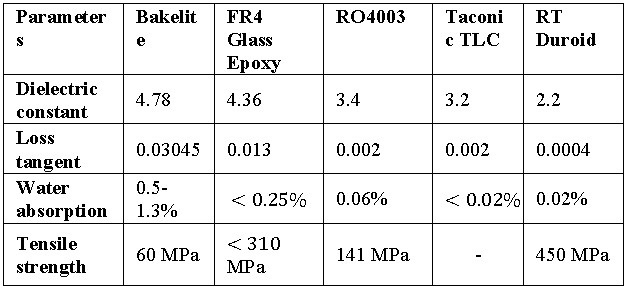
\includegraphics[width=.75\textwidth]{figures/Yannis/substrate.jpg}
\caption{Properties of different substrates. \cite{substrates}}
\label{substrate}
\end{figure}

\begin{table}[ht]
\centering
\begin{tabular}[width=.75\textwidth]{| c | c | c | c | c | c |}
\hline
 - & \textbf{Bakelite} & \textbf{FR4 Glass Epoxy} & \textbf{RO4003} & \textbf{Taconic TLC} & \textbf{RT Duroid} \\ 
 \hline
 \textbf{$\epsilon_{r}$} & 4.78 & 4.36 & 3.4 & 3.2 & 2.2 \\  
 \hline
 \textbf{L (mm)} & 290.9 & 305.2 & 336.9 & 344.8 & 395 \\
 \hline
 \textbf{W (mm)} & 202.7 & 215.3 & 244.2 & 251.7 & 301.8 \\
 \hline
\end{tabular}
\caption{Patch antenna's dimensions for different dielectric constant $\epsilon_{r}$. f=300 MHz}
\label{table: subs300}
\end{table}

\begin{table}[ht]
\centering
\begin{tabular}[width=.75\textwidth]{| c | c | c | c | c | c |}
\hline
 - & \textbf{Bakelite} & \textbf{FR4 Glass Epoxy} & \textbf{RO4003} & \textbf{Taconic TLC} & \textbf{RT Duroid} \\ 
 \hline
 \textbf{$\epsilon_{r}$} & 4.78 & 4.36 & 3.4 & 3.2 & 2.2 \\  
 \hline
 \textbf{L (mm)} & 216.4 & 228.9 & 252.7 & 258.6 & 269.3 \\
 \hline
 \textbf{W (mm)} & 150.3 & 161.3 & 183 & 188.6 & 226.1 \\
 \hline
\end{tabular}
\caption{Patch antenna's dimensions for different dielectric constant $\epsilon_{r}$. f=400 MHz}
\label{table: subs400}
\end{table}

Knowing from antenna theory that the radiating slots of a patch antenna can be seen as two independable dipoles, we can use this approximation to find the gain using the array factor (AF). If we assume a assume a dielectric constant, which compromise size and efficiency, we can choose the RO4003 from \ref{table: subs300} or \ref{table: subs400}. Thus, if the area below our lander vehicle is 1 $m^2$ we can design a 6 element patch array antenna with element's size 377x244 mm if we are go for the lower frequency of 300 MHz. According to Balanis' approximated formulas we can have directivity for each slot equal to 4 dB and around 5.8 dB for the whole antenna (two slots). In order to increase the directivity using the array design of 6 elements we can achieve a half power beamwidth about $40^{\circ}$, as it can be seen in figure (\ref{array}). In case we design the antenna for 400 MHz, the patch size will be smaller, thus more antennas can be placed to the available space. Always we have to consider that higher frequencies correspond to higher losses and in case of patch antennas without any substantial increase in gain and beamwidth.

\begin{figure}[ht]
\centering
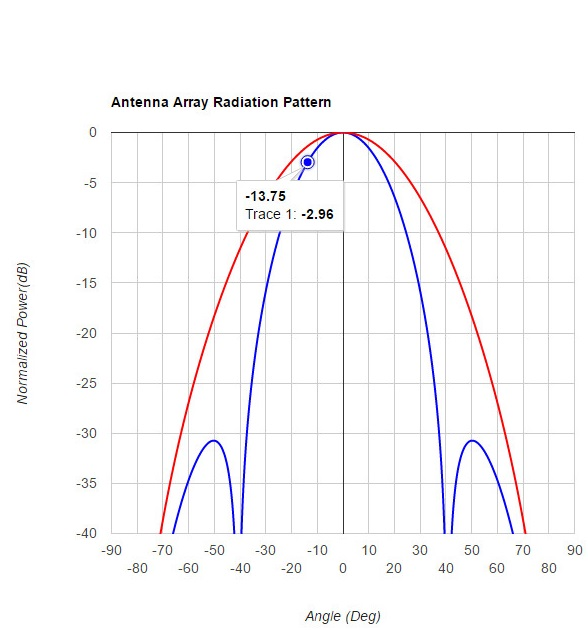
\includegraphics[width=.75\textwidth]{figures/Yannis/2results.jpg}
\caption{Half power beamwidth for an antenna array of 6 microstrip antennas (red curve) and for an antenna array of 12 microstrip antennas (blue curve). Both are pointing at broadside.}
\label{array}
\end{figure}

Finally, in order to determine the the gain we have to know the radiating efficiency. As it has stated, taking into account the absence of the necessary dedicated software for antenna analysis, such as HFSS and CST, we are trusted the results from \cite{substrates} as they are shown in figure (\ref{array result}). The last step is to find the gain of the antenna. The designing characteristics of the aforementioned antenna of 6 elements are summing up in table (\ref{table: results}).

\begin{figure}[ht]
\centering
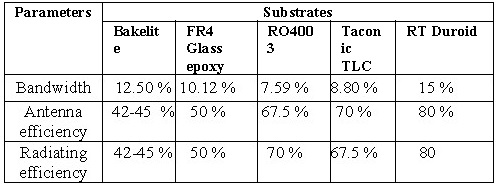
\includegraphics[width=.75\textwidth]{figures/Yannis/results.jpg}
\caption{Fractional bandwidth, antenna efficiency and radiating efficiency for a single patch antenna. The measurements reported in \cite{substrates} correspond to frequency 10 GHz, although due to poor dependence of these quantities from frequency we can use them for our approximations.}
\label{array result}
\end{figure}

\begin{table}[ht]
\centering
\begin{tabular}{| c | c | c | c | c | c | c | c |}
\hline
 \textbf{f (MHz)} & \textbf{$\epsilon_{r}$} & \textbf{W (mm)} & \textbf{L (mm)} & \textbf{D (dB)} & \textbf{$\epsilon_{rad}$} & \textbf{G (dB)} & FBW \\ 
 \hline
 300 & 3.4 & 244 & 337 & 5.76 & 70 \% & 4.03 & 7.59 \% \\
 \hline
 400 & 3.4 & 183 & 252 & 9.4 & 70 \% & 6.58 & 7.59 \% \\
 \hline
\end{tabular}
\caption{Design characteristics for a patch antenna array. 300 MHz corresponds to 6 elements array and 400 MHz to 12 elements. D stands for maximum directivity and G for maximum gain.}
\label{table: results}
\end{table}

An important part of microstrip antennas (and especially in arrays) is the input impedance and matching. The input admittance of a slot and thus for a patch antenna is given by using Huygens's equivalent principle. The procedure is quite laborious and will not be shown here. Although, a useful consequence is that we can match the input admittance by a very easy technique, using a small inset in each individual patch. Also, if circular polarization is needed many different techniques of feeding can be used. Of course, since we are talking for an array antenna, the appropriate phase differences should be introduced between the array elements. About feeding we can use either uniform or nonuniform antennas, which mean constant or varying magnitude of the elements. Non-uniform arrays are more preferable since they present lower sidelobe and grating lobe levels, but on the other hand worst directivity. Good cases for non-uniform amplitude coefficients are the binomial and Tschebysheff's polynomial. 

\subsection{Penetrator Antenna}

As it was mentioned in \ref{microstrip antenna}, the great advantage of patch antennas are their compact size. Having in mind the extremely limited available space at penetration vessel to place an antenna, the option of a patch antenna or a small array of them seems a good alternative. The analysis is exactly the same as it was done previously, so only minor modifications are necessary. First of all, array's elements must be placed on the sides of the vessel due to limited area on the top. Moreover, the antenna design must be an end-fire, which means that the antenna beam points along the axis where the elements are placed, thus the desired beam will point at $\theta=0$. In order to achieve that properly phase difference should be introduced to the elements. The positive side of that is the possibility of redirecting the beam in case of misalignment between penetrating vessel and lander vehicle antenna. Taking into account the size of the vessel, approximately 10-15 cm outer diameter, the patch antennas should be placed around its periphery. 

\begin{table}[ht]
\centering
\begin{tabular}{| c | c | c | c | c | c | c | c |}
\hline
 \textbf{f (MHz)} & \textbf{$\epsilon_{r}$} & \textbf{W (mm)} & \textbf{L (mm)} & \textbf{D (dB)} & \textbf{$\epsilon_{rad}$} & \textbf{G (dB)} & FBW \\ 
 \hline
 300 & 3.4 & 244 & 337 & 4.45 & 70 \% & 3.12 & 7.59 \% \\
 \hline
 400 & 3.4 & 183 & 252 & 7.12 & 70 \% & 4.86 & 7.59 \% \\
 \hline
\end{tabular}
\caption{Design characteristics for a patch antenna array of penetrator vessel. 300 MHz corresponds to 3 elements array and 400 MHz to 5 elements. D stands for maximum directivity and G for maximum gain.}
\label{table: results_pen}
\end{table}

\subsection{Link Budget Analysis}

The link budget will take place in this section, in order to assess which one of the above configurations is most suitable for our application. In this part we are interested in high directional link with the best possible efficiency and lower possible size, taking into account the ice losses with relation to frequency. Moreover, the necessary data rate should be kept in mind. As it has mentioned above, the period of the orbiter around Europa is approximately 13 days, which means penetrator vessel sends data to the lander vehicle during this period and the latter stored there, until the next pass of the orbiter. The available time, when line of sight between ground and space segment will have been established longs only few hours (around 3 hours), thus we have to deliver any stored data from 13 days in this small interval. This is our main driver concerning data rates and it limits the uploaded data size to 1 Gbit (giga bit) in three hours. Consequently, we can calculate the necessary data rate between penetrator-orbiter should be 1 Kbps (kilo bit per second) to achieve 1 Gb accumulation in 13 days. Although, if demand for higher data rates occurs, we can push the limits of our equipment compromising the signal to noise ratio.

The following link budget calculations are based on Friis formula of propagation, taking into account propagation losses due to the distance (distance in worst case scenario is 10 Km), losses due to ice, as described in \ref{losses}, losses from different components (transmission lines, tranceivers, etc.) and polarization mismatches. Due to indeterministic nature of ice losses, two average estimation will be included in the calculations. The first will be an estimated worst case scenario with ice losses of 8 dB/Km and an intermediate case scenario with 6 dB/Km. Finally, for each different antenna design, the link budget with a 1 dB required $E_{b}/N_{0}$ will be found and then an overall estimation will take place. 

\begin{table}[ht]
\centering
\begin{tabular}{| c | c | c | c | c | c |}
\hline
 \textbf{Ant. Type} & \textbf{$G_{Tx}$ } & \textbf{$G_{Rx}$ } & \textbf{Add. Losses } & \textbf{Pol. Losses} & $E_{b}/N_{0} $ \\ 
 \hline
 Crossed-Yagi & 8.6 dB & 3.12 dB & 0.5 dB & 3 dB & 5.4 dB \\
 \hline
 LPDA & 7 dB & 3.12 dB & 0.5 dB & 3 dB & 3.8 dB\\
 \hline
 Helical & 7.8 dB & 3.12 dB & 0.5 dB & 0 dB & 7.6 dB\\
 \hline
 Parabolic & 7.2 dB & 3.12 dB & 0.5 dB & 0 dB & 7 dB\\
 \hline
 Microstrip & 4 dB & 3.12 dB & 0.5 dB & 0 dB & 3.8 dB\\
 \hline
\end{tabular}
\caption{Link budget analysis for the different types of antennas, at frequency of 300 MHz, for the worst case scenario attenuation due to ice losses (8 dB/km). The computations take into account the dielectric constant of the ice, bit rate of 1 Kbps and transmitted power of 10 Watts. The distance which is calculated is 10 km of ice with impurities.}
\label{table: link_budget}
\end{table}

\subsubsection{Link Budget Analysis \& Feasibility Assessment}
\paragraph{Yagi \& LPDA antennas}
Table \ref{table: link_budget} is a link budget analysis which concentrates on telecommunication characteristics. Beside them we have to take into account also dimensions and the corresponding beamwidth in any case to find out the most suitable antenna, the number of elements/turns, array factor, etc. As mentioned earlier, Yagi and LPDA antennas are quite efficient, but on the other hand they take more space because of the necessary distance between the elements and need a sufficient distance from the first "obstacle" in the near field, ice in our case. Moreover, there is an extra 3 dB loss, due to polarization mismatches in order to be able to receive/transmit circular polarization. These reasons are enough to not consider Yagis and LPDAs as our first priority. 
\paragraph{Helical antennas}
Helical antennas are quite promising not only because of their very good gain and efficiency, but also for their extremely good beamwidth in this frequency range. Another advantage of them is the ability to built a planar array, with small footprint, in order to increase the gain and decrease the beamwidth. Finally, we can manipulate each element independently, which provides more freedom to our design. After the above, we can see from  tables \ref{table: Helicals1} and \ref{table: Helicals2} that there are substantial differences between the frequencies and the use of an array of helical antennas. Having in mind the strict limitation of space under our lander vehicle, the most suitable helical antenna is around 340 MHz and N=3 (table \ref{table: Helicals2}). This specific design is a compromise between long antennas, high gain, sufficient beamwidth to consider the antenna directional and fairly low frequency to avoid high ice losses. It is also noticeable that the single element exceeds the performance of an array, which is not strange in these frequencies. We could choose also the respective antenna at 400 MHz, but the increase of ice losses at 400 MHz are far higher than the almost 1 dB extra gain. Last but not least, this design has the advantage that can be folded and unfolded easily. We can have the coil compressed and attached to a wire, in order to provide the necessary tension to keep it folded. When we want to deploy the antenna we will need only a resistor and a very small current to produce some heat and melt the wire, thus our antenna will be deployed as a reaction.
\paragraph{Parabolic/Dish antennas}
Parabolic antennas can approach very good efficiencies and provide the necessary gain. Their diameter and shape can fit below our vehicle, although it will be more difficult to fold and unfold this design comparing with helical antennas. Additionally, as it can be seen (table \ref{table: dish}) the beamwidth at the same frequencies as helicals, is much wider, thus these antennas are less directive. The above mentioned reasons are sufficient to exclude this design. 
\paragraph{Microstrip Antennas}
Microstrip antennas are well suited when space is high priority with the expense of low quality and small gain. Microstip antennas at 300 MHz present a gain only 4 dB, which cannot be compared with the other designs. Although, their inefficiency can be overlooked in the case of the penetrator vessel where the absence of space does not leave any other option.

Finally, the link budget for the proposed antenna (helical), in the frequency of 340 MHz and with N=3 is shown in table \ref{table:link_budget_helix}.

\begin{table}[ht]
\centering
\begin{tabular}{| c | c | c | c | c | c |}
\hline
 \textbf{Ant. Type} & \textbf{$G_{Tx}$} & \textbf{$G_{Rx}$} & \textbf{Add. Losses} & \textbf{Pol. Losses} & \textbf{$E_{b}/N_{0}$} \\ 
 \hline
 Helical & 17.7 dB & 3.12 dB & 0.5 dB & 0 dB & 17.5 dB \\
 \hline
\end{tabular}
\caption{Link budget analysis for a helical antenna, at frequency of 340 MHz, for the worst case scenario attenuation due to ice losses (8 dB/km). The computations take into account the dielectric constant of the ice, bit rate of 1 Kbps and transmitted power of 10 Watts. The distance which is calculated is 10 km of ice with impurities.}
\label{table:link_budget_helix}
\end{table}

\subsection{Implementation's hazards}
As discussed in this section, directivity is a desirable characteristic of antennas when you want to concentrate the beam in a specific direction. Nevertheless, in some cases high directivity can lead to mission failure, especially when the "target" object changes direction rapidly. In our application this is not the case, but misalignments can occur because of different unexpected factors. For instance, while the penetrator will be melting the ice, the heat may not propagating isotropically, thus gradually the penetrator will start diverging from the expected route. If we do not foresee the capability of beam steering and the deviation become large, there is possibility to lose the penetrator vessel from our "field of view". In other cases, may will be desirable to change the route of our penetrator to avoid obstacles, such as rocks, liquid pools, etc. In either cases, we must have the possibility to steer the beam or change its beamwidth in such manner to retain the communication.

Another problem which is possible to come across is the landing on a steep slope, instead of a relative smooth area. In the former case, we must built the antenna under the lander vehicle in order to be able to point at different directions and not only perpendicular to vehicle's surface, as shown in figure \ref{ant steer}. This can be done by placing the antenna onto a steerable ground plane or by steering only the antenna's coil without moving the ground plane. The latter case will result in a slightly squinted beam with respect to the normal unit vector of ground plane, but if we know the desired direction we can compensate for this misalignment, in order to achieve the maximum directivity.

\begin{figure}[ht]
\centering
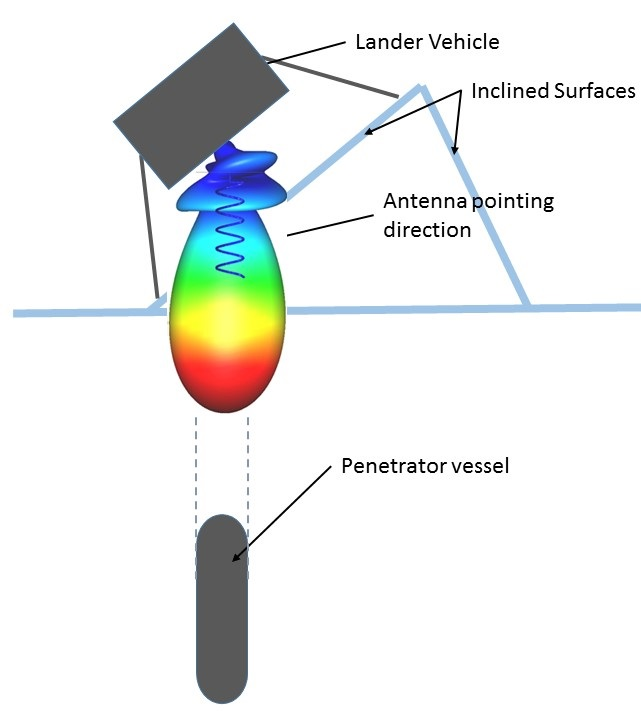
\includegraphics[width=.6\textwidth]{figures/Yannis/normal.jpg}
\caption{The antenna beam must point at penetrator vessel, even if the landing take place at an inclined surface.}
\label{ant steer}
\end{figure}
 %Isn't this supposed to be a subsection of the penetrator to lander link?

\autsection{Communication Systems Proposal}{Kristian Sloth Lauszus, Rasmus Lundby Pedersen, and Gustavo Feijóo Carrillo}

==== Trans Ice Communications Presentation
    -Fiber optical cables are heavy.
    -Repeaters require RTGs with a high interval. Number of repeaters is highly depending on ice conditinos
    -One-to-one communication link through the ice is a better alternative.
CONCLUSION: Fiber optical cable is not a good option, cable is going to be enormous.
            One-to-one communication must be researched further - more details are required.
            Repeater communication must be researched further.
            
==== Communications Presentation
-Ice link:
-Surface relay:
-Ground control link:
One-to-one communication, assuming poor ice conditions, link is possible
Surface to orbiter. Small tracking possibilities, low directivity antenna is used.
3m high gain antenna.
CONCLUSION: One-to-one communication must be researched further. More details are needed
            The antenna transmitting down through the ice must be aligned. High risk, as landing site will probably not be flat.

* Repeaters along decent path
	* Increases a lot when introducing salinity
	* Pros:
		* Scalable
	* Cons:
		* Complexity
		* Separate RTGs
	* Too complex
		* Better just use one proper designed unit in the penetrator
		* Might be a combinations of repeaters and a big antenna at the lander and probe
		* Will also work better if the probe doesn't move straight

	* Also a combination of repeaters and tether could be used.
	* The repeater will also work better if the penetrator move to the side. Repeaters do not risk breaking like the tether.
	* If one repeater fails the data rate will drop by a factor 10 or more, so we have a little redundancy.
